\documentclass[a4paper]{scrartcl} 
\usepackage[utf8]{inputenc} 
\usepackage{ngerman}
\usepackage{graphicx} 
\usepackage[plainheadsepline,headsepline,footsepline]{scrlayer-scrpage}
\usepackage[margin=3cm]{geometry}
\usepackage{lastpage}
\usepackage{xspace}
\usepackage{datatool}
\usepackage{fancybox}
\usepackage{siunitx}
\usepackage{placeins}
\usepackage{float}
\usepackage{subfigure}
\usepackage{ulem}
\usepackage{url}
%\usepackage{hyperref}

\renewcommand{\familydefault}{\sfdefault}

%Deklaration der Variablen
\newcommand{\aw}{Hinweise zum Aufbau}		%Arbeitsanweisung, Wartungsanweisung,etc.
\newcommand{\DocNr}{V0.2a {\scriptsize DE}}			%Bezeichnung der Arbeitsanweisung
\newcommand{\tit}{Hector 9000}	 		%Titel
\newcommand{\rev}{V0.2a DE}				%Revisionsnummer
\newcommand{\er}{Cadmium, kater, Marv}		%Erstellt von
\newcommand{\stand}{2018-10-30}		%Letzte Revision
\newcommand{\stat}{ENTWURF!}			%Status: Entwurf, kontrolliert, freigegeben, obsolet...

\pdfinfo{ /Author (\er) /Title (\aw \rev \tit) }

%Definition Headings 
\pagestyle{scrheadings}		% default-Pagestyle
\lohead*{\aw}
\cohead*{\textbf{\tit}}
\rohead*{
\includegraphics[width=2cm,trim=0 18mm 0mm 0]{pics/Logo.png}}
\lofoot*[]{\DocNr}
\cofoot*[]{\stand}
\rofoot*[]{\thepage/\pageref{LastPage}}

\setkomafont{pageheadfoot}{}		% kein slanted Font

%Definition Titelseite
\title{ ~\\[2cm] {\Huge\tit} \\ {\aw}}
\author{\er}
\date{\small \DocNr{} vom \stand} 


%%%% Dokument
\begin{document}
\maketitle
\vspace*{\fill} % legt den Abstract ans untere Ende der Seite
\begin{abstract}
\noindent
Hector 9000 ist ein Cocktailautomat, der 12 verschiedene Getränke dosieren kann. Entstanden ist Hector 9000 Anfang 2018 als Nachfolger von Onkel Hector, einem reinen Gin-Tonic-Automaten. Bei der Entwicklung wurde versucht, möglichst viele Teile durch 3D-Druck, ohne Support, herzustellen.\\
Im Gegensatz zu vielen anderen Barbots werden keine Peristaltikpumpen verwendet, wodurch eine Förderung von kohlensäurehaltigen Getränken möglich ist. Die Flüssigkeiten werden durch einen leichten Überdruck in den Flaschen gefördert, gleichzeitig wird die geförderte Menge durch eine Waage ermittelt. Ist genug von einem Getränk dosiert worden, werden die zum Getränk gehörigen Silikonschläuche abgequetscht. Die Getränke kommen dabei nicht mit beweglichen Teilen in Berührung. Ist ein Cocktail fertiggestellt, betätigt Hector seine Glocke.\\
Das Herz von Hector 9000 ist ein Raspberry Pi 3B. Der Pi übernimmt die Ablaufsteuerung und stellt auf einem 7''-Touch-Display das UI dar.
Die Software ist in Python~3 geschrieben, zur grafischen Darstellung wird Kivy genutzt.
\end{abstract}

%\thispagestyle{scrheadings}

\FloatBarrier
\newpage
\tableofcontents

\listoffigures

\listoftables
\newpage

\section{Haftungsausschluss}
Wir übernehmen keinerlei Verantwortung für Verletzungen oder Schäden, die beim Nachbau und Betrieb von Hector 9000 entstehen. 

\section{Hardware}
\subsection{Mechanik}

\subsubsection{Waage}
Um die dosierten Mengen zu ermitteln, wird eine Wägezelle in Verbindung mit einem HX711 verwendet. Vor der Montage der gedruckten Kunststoffteile muss der Überlauf in die Waagschale eingeklebt werden. Die Befestigung der Waage erfolgt von oben durch die Tischplatte. Der Abstandshalter und der Überlauf müssen abhängig von der Dicke der Tischplatte angepasst werden, zwischen Tischplatte und Waagschale sollte ein Spalt von \SI{1}{\milli\metre} sichbar sein. Als Anschlusskabel wurde ein CAT5e-Kabel verwendet. Auf der Unterseite des Gehäuses besteht die Möglichkeit, einen Schlauch mit \SI{10}{\milli\metre} Innendurchmesser für den Überlauf anzuschließen. Für die Montage der Waage hat sich folgende Reihenfolge bewährt:

\begin{enumerate}
  \item Kabelverschraubung im Gehäuse befestigen,
  \item Gehäuse und Wägezelle unter der Tischplatte positionieren,
  \item Wägezelle von oben anschrauben,
  \item Abstandshalter und Waagschale befestigen,
  \item Kabel verlöten,
  \item Deckel verschrauben.
\end{enumerate}

\begin{figure}
  \centering
  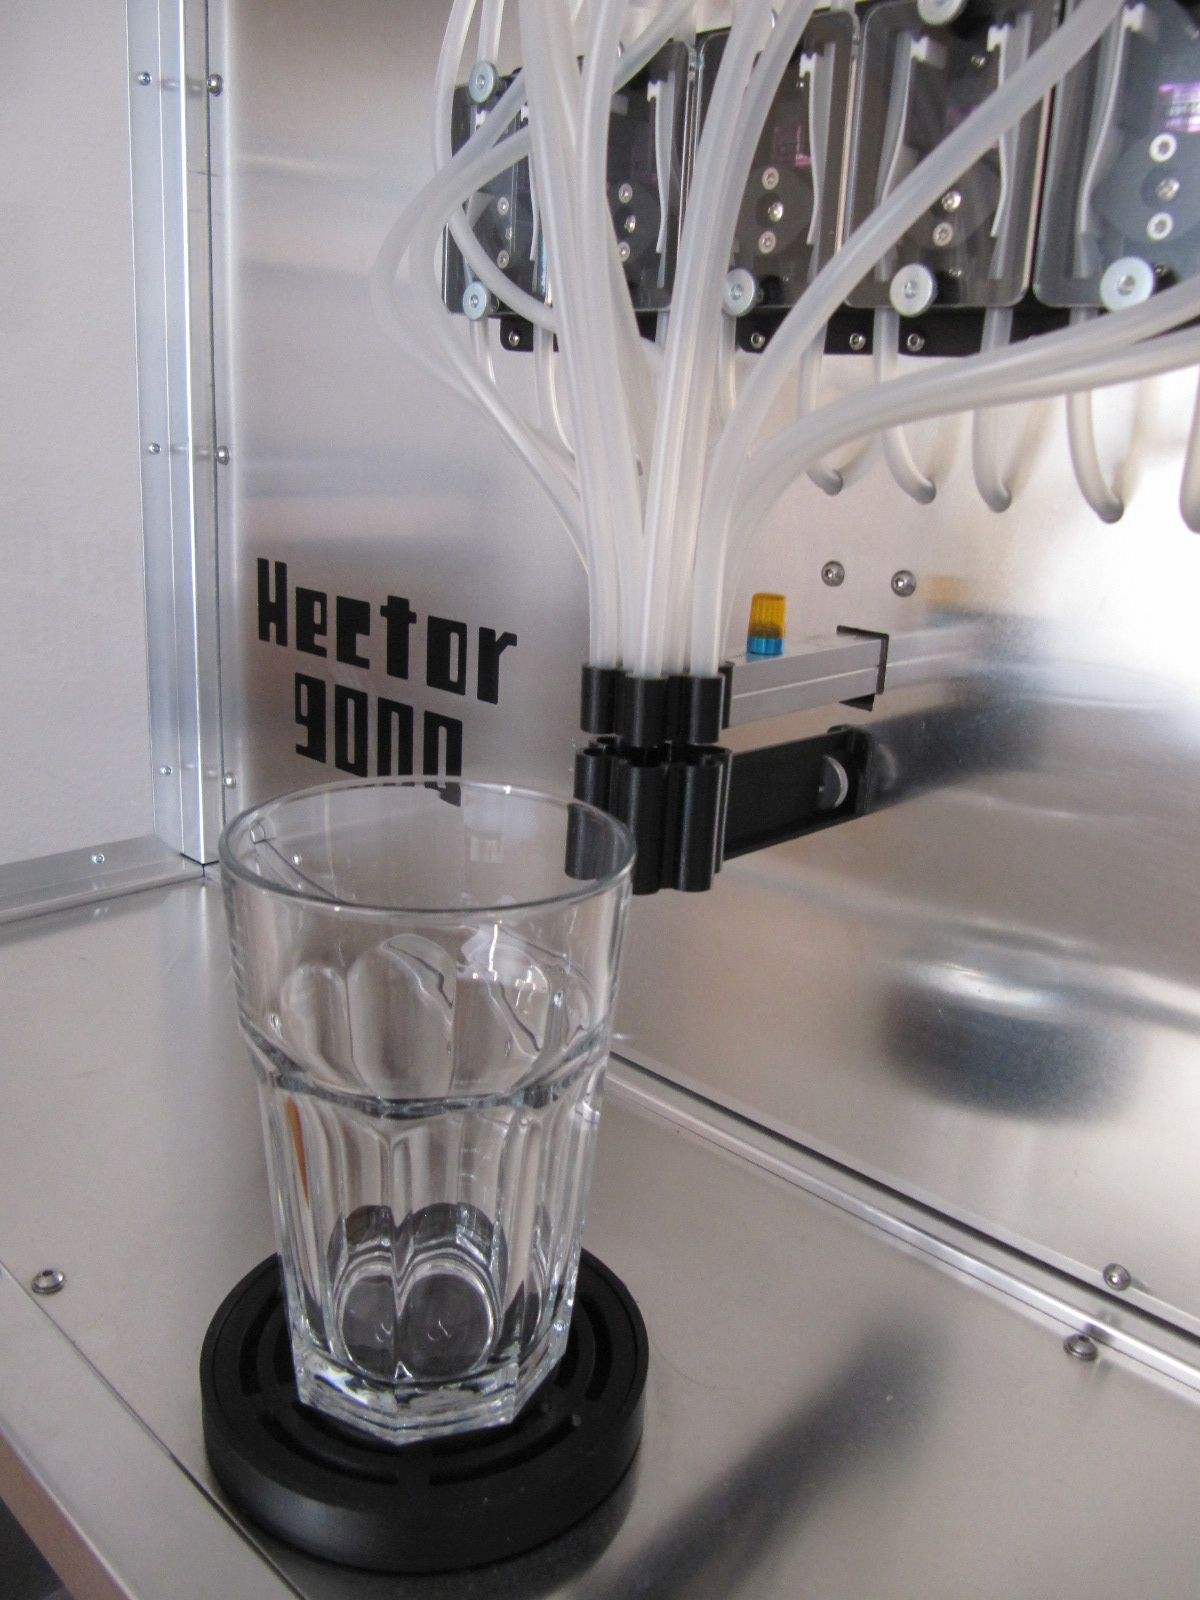
\includegraphics[height=8cm]{pics/scale_glass.JPG}
  \caption{Waage mit Glas} \label{scale_glass}
\end{figure}

\begin{figure}
  \centering
  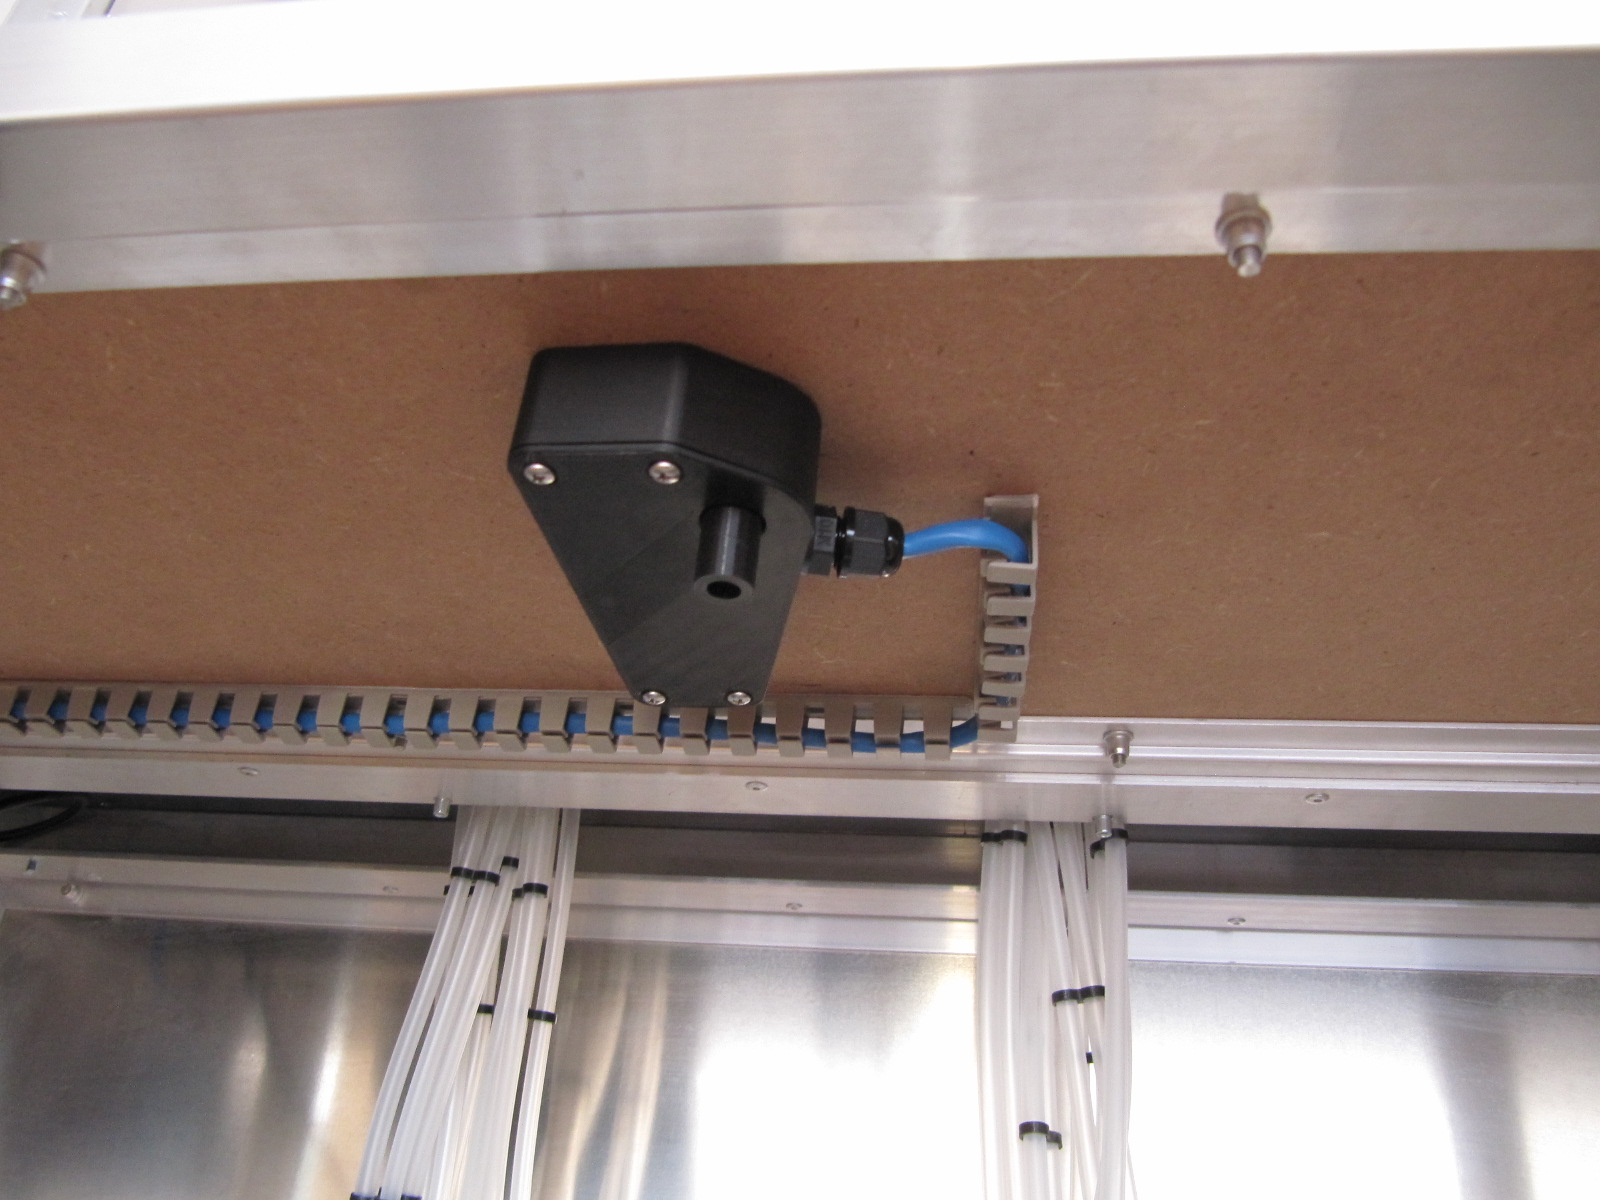
\includegraphics[height=8cm]{pics/scale_bottom.JPG}
  \caption{Waage von unten}
\end{figure}
  
\subsubsection{Pumpe}
Um den Überdruck in den Flaschen zu erzeugen, verwenden wir eine Luftpumpe für Aquarien. Da die komplette Elektronik mit max.~12\,VDC laufen soll, haben wir uns für eine 12V-Pumpe von Schego entschieden. Die Auswahl der Pumpe ist relativ unkritisch, da der benötigte Überdruck und die Fördermenge gering sind. Es sollte lediglich darauf geachtet werden, dass die Pumpe ölfrei arbeitet. Da die Pumpe nur über ein einziges Loch zur Befestigung verfügt, wurde eine Halterung konstruiert. Folgende Reihenfolge bei der Montage hat sich bewährt:

\begin{enumerate}
  \item Jeweils an einem Ende der Gewindestangen 2 Muttern aufschrauben und kontern. Eine Mutter sollte bündig mit der Gewindestange abschließen, die Schlüsselflächen der Muttern müssen in einer Flucht stehen.
  \item Gewindestangen in die dafür vorgesehenen Löcher stecken,
  \item Halterung im Gehäuse festschrauben,
  \item Pumpe einsetzen und mit den U-Profilen festklemmen (optional mit Moosgummistreifen unter den U-Profilen),
  \item Muttern an den U-Profilen kontern oder mit Loctite verkleben.
\end{enumerate}

\begin{figure}
  \centering
  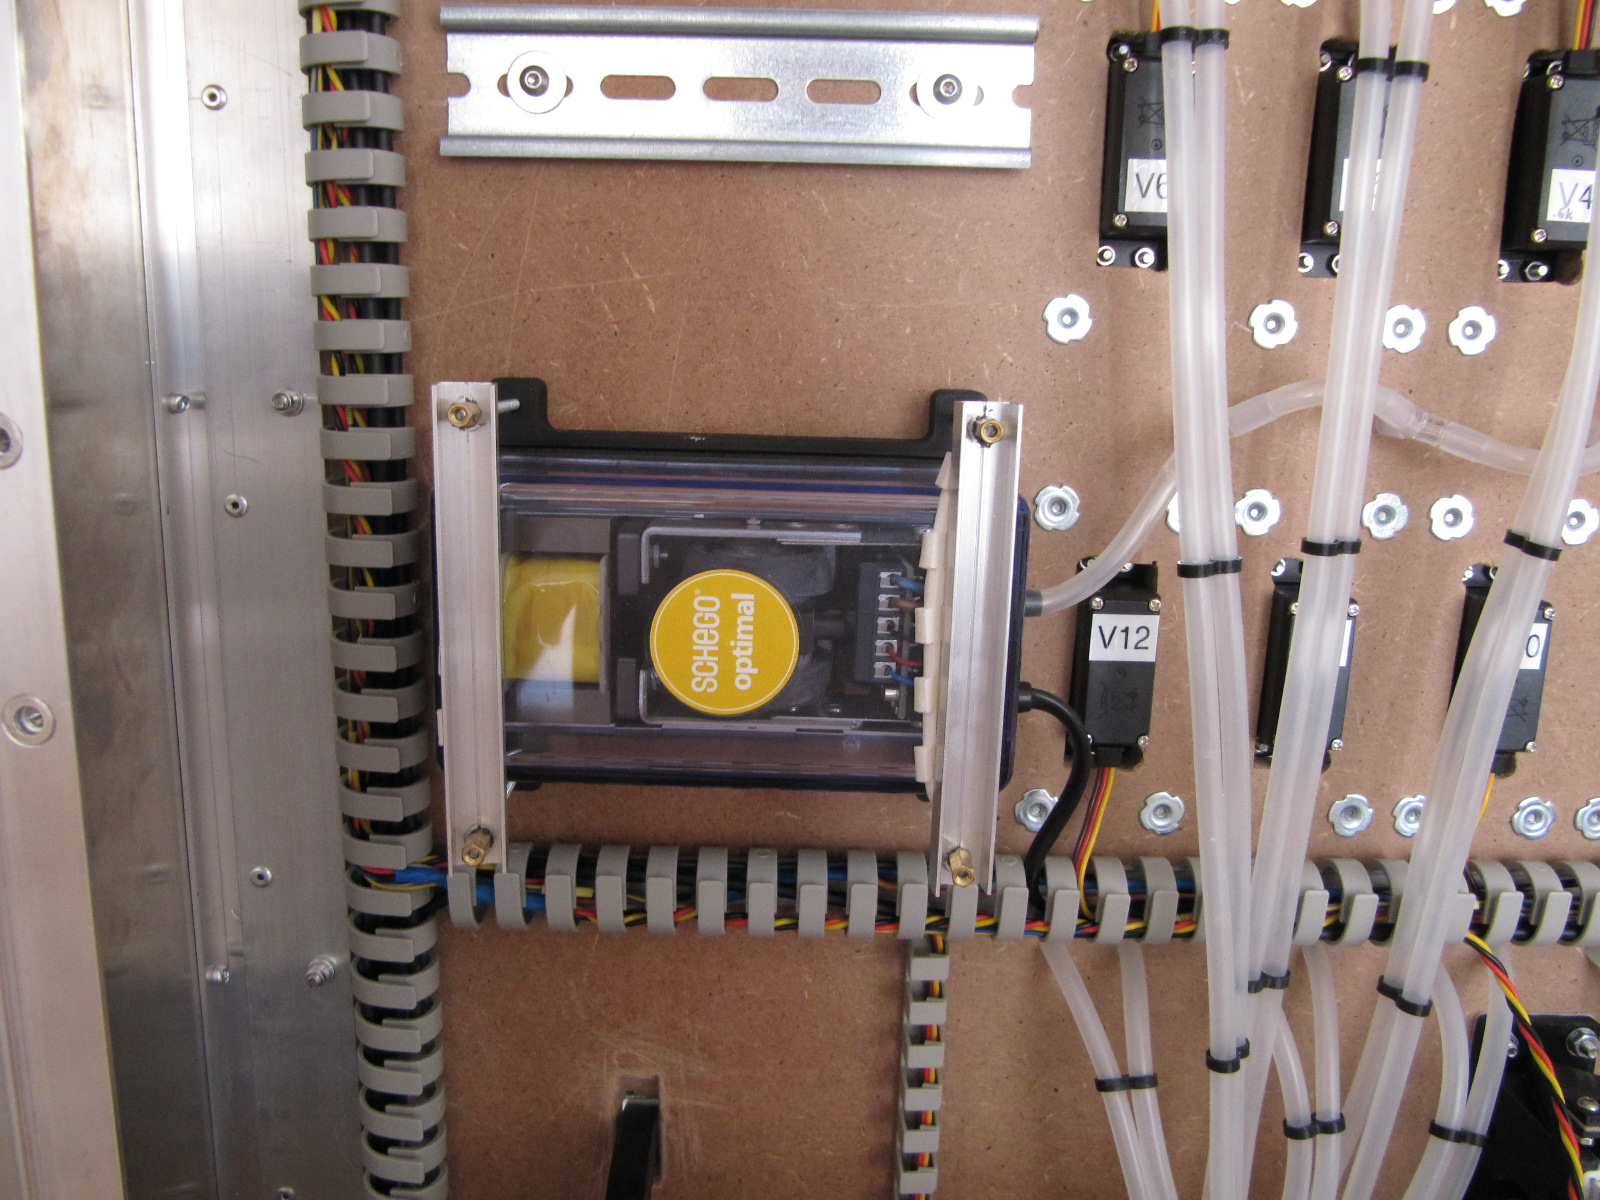
\includegraphics[height=8cm]{pics/pump.JPG}
  \caption{Luftpumpe} \label{pump}
\end{figure}
\newpage

\subsubsection{Ventile}
Um die Dosierung der Flüssigkeiten zu realisieren, wurden für unseren Cocktailautomaten Quetschventile konstruiert, welche immer beide Schläuche (Luft \textit{und} Flüssigkeit) einer Zutat  gleichzeitig öffnen bzw. schließen. \\
Die benötigten Kunststoffteile für die Ventile können ohne Support gedruckt werden. Die (optionale) Abdeckung wurde für unseren Automaten mit einem CO\textsubscript{2}-Laser aus transparentem PMMA geschnitten.
Es ist darauf zu achten, dass die Servos originale \textit{TowerPro MG996R} sind. Es gibt Servos mit gleicher Bezeichnung von No-Name-Anbietern, aber diese Servos können sich in den Außenabmessungen teilweise erheblich von den originalen Servos unterscheiden. 
Die bei den Servos mitgelieferten runden Servoarme müssen auf den Innendurchmesser der Nocken angepasst werden. Hierbei ist besondere Sorgfalt notwendig: Sitzen die Servoarme exzentrisch im Nocken, wird das Ventil nicht richtig absperren. Unsere Servoarme wurden auf einer CNC-Fräse mit einem sehr scharfen Holzfräser bearbeitet. Die Befestigungslöcher für die Servoarme werden am besten gebohrt, indem der Nocken als Schablone genutzt wird. Die Schrauben zur Verbindung von Nocken und Servoarm werden mit Loctite gesichert. 
Bei den Zungen ist darauf zu achten, dass sie aus einem Material mit guten Gleiteigenschaften gefertigt werden. Unsere Zungen wurden aus \textit{Iglidur I150} gedruckt. Die Zungen in den Ventilen von Onkel Hector haben schon einige hundert Zyklen hinter sich und funktionieren immer noch einwandfrei. Alternativ könnten die Zungen aus PET gedruckt werden, dies wurde allerdings noch nicht getestet. 
Damit die Ventile bündig mit der Rückwand sitzen, müssen Auschnitte für die Servos hergestellt werden (Abb. \ref{valve_rear}). Zur Befestigung der Ventile haben sich Einschlagmuttern bewährt. 

\begin{figure}
  \centering
  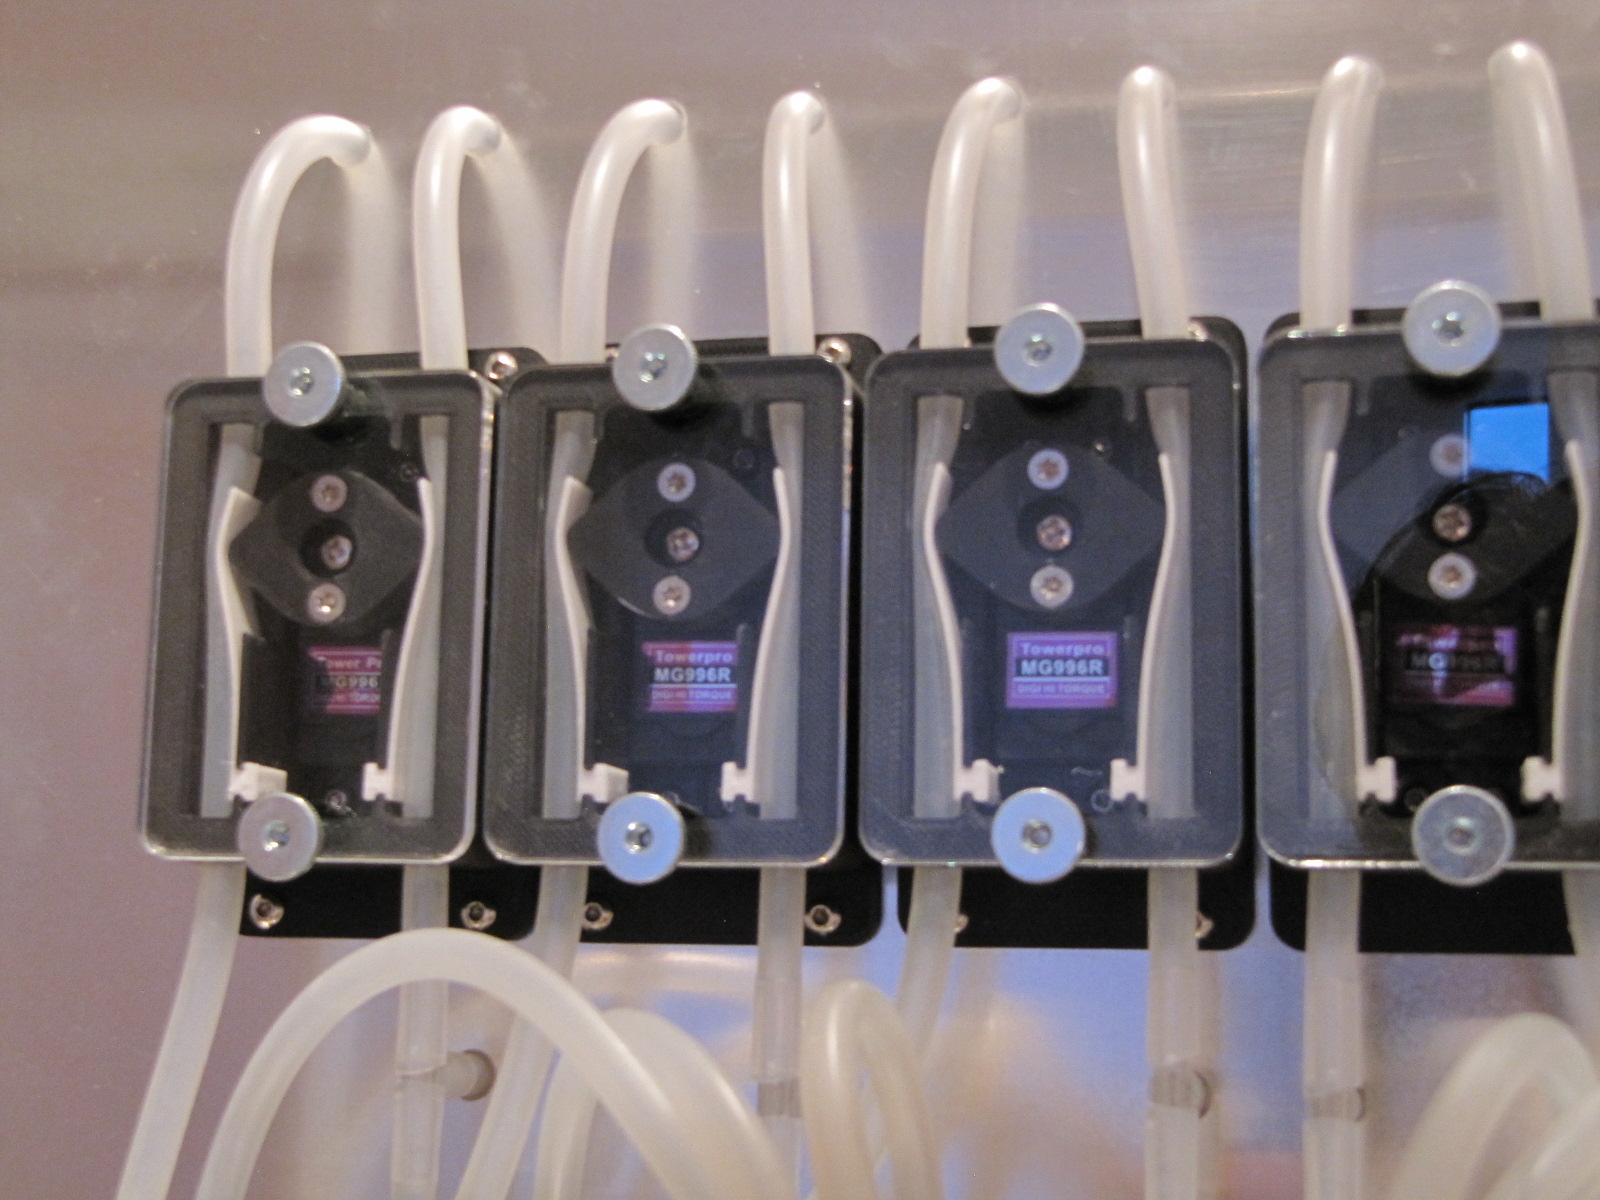
\includegraphics[height=8cm]{pics/valve_front}
  \caption{Ventile} \label{valve_front}
\end{figure}

\begin{figure}
  \centering
  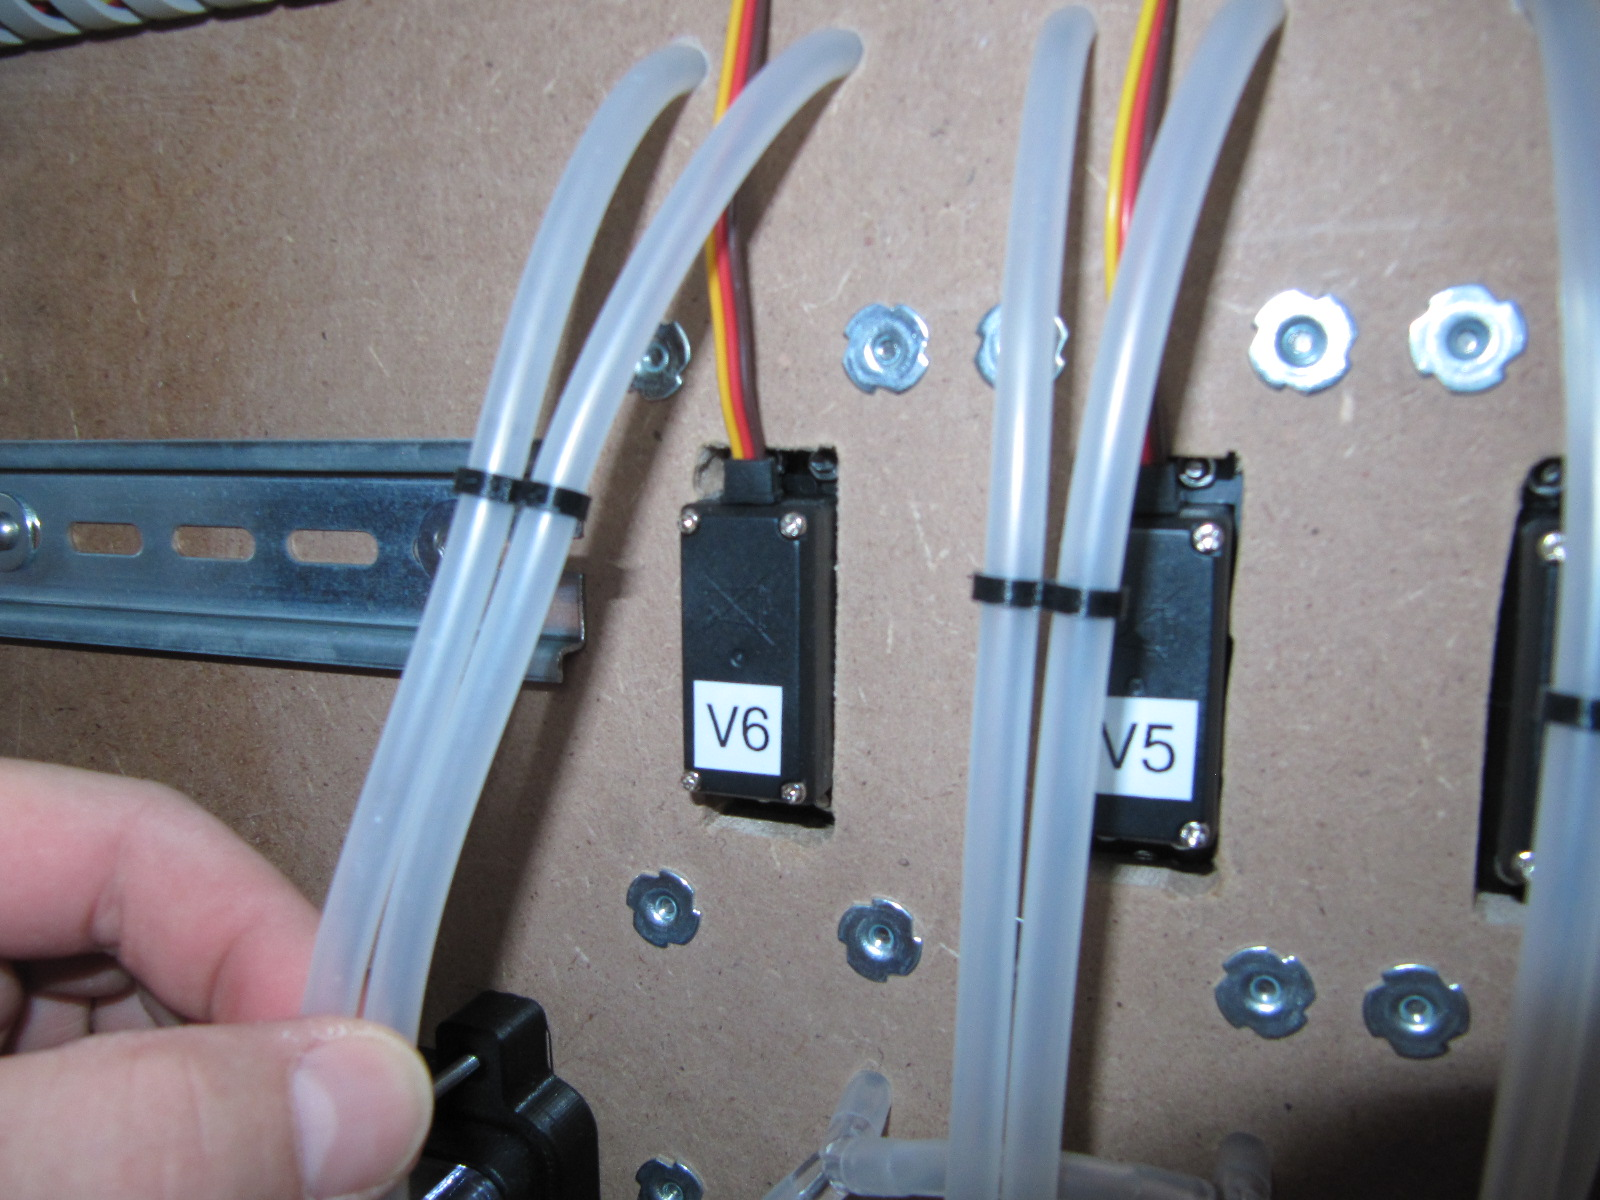
\includegraphics[height=8cm]{pics/valve_rear}
  \caption{Ventile von hinten} \label{valve_rear}
\end{figure}

\subsubsection{Arm}
Um den Füllvorgang komfortabler zu gestalten, ist der Arm mit dem Dosierkopf im Normalzustand eingefahren (Abb. \ref{arm_front_in}). Wird der Dosiervorgang gestartet, fährt der Arm nach vorne. Alle benötigten Kunststoffteile lassen sich ohne Support drucken. Der Gleiteinsatz sollte aus einem Material mit guten Gleiteigenschaften gefertigt werden. Unser Gleiteinsatz wurde aus \textit{Iglidur I150} gedruckt. Alternativ könnte der Gleiteinsatz aus PET gedruckt werden, dies wurde allerdings noch nicht getestet. Der Ausleger besteht aus einem Aluminiumprofil mit \SI{15.5}{\milli\metre} Kantenlänge. Solche Profile sind in fast jedem deutschen Baumarkt zu finden. Das Ritzel wird auf die Welle des Motors gepresst und braucht keine weitere Sicherung. Um die Zahnstange an dem Ausleger zu befestigen, wurden M3-Blindnietmuttern in das Profil eingesetzt. Der Dosierkopf wird mit einer selbstschneidenden Schraube im Profil gesichert. Der Auslöser wird mit dem Ausleger verklebt. Der Auslöser weist ein Loch auf. Durch dieses Loch wurde ein Kabel geführt, um ein optionales Rundumlicht auf dem Arm mit Strom zu versorgen.\\
Bei der Montage des Arms ist darauf zu achten, dass die untere Schraube von hinten durch die Bohrung geführt und mit einer regulären Mutter festgeschraubt wird. Die oberen Schrauben werden von vorne durch die Rückwand gesteckt und verschraubt. Auf der unteren Schraube kann nun mit einer Rändelmutter der Tropfenfänger montiert werden (Abb. \ref{drip}).  

\begin{figure}[H]
  \centering
  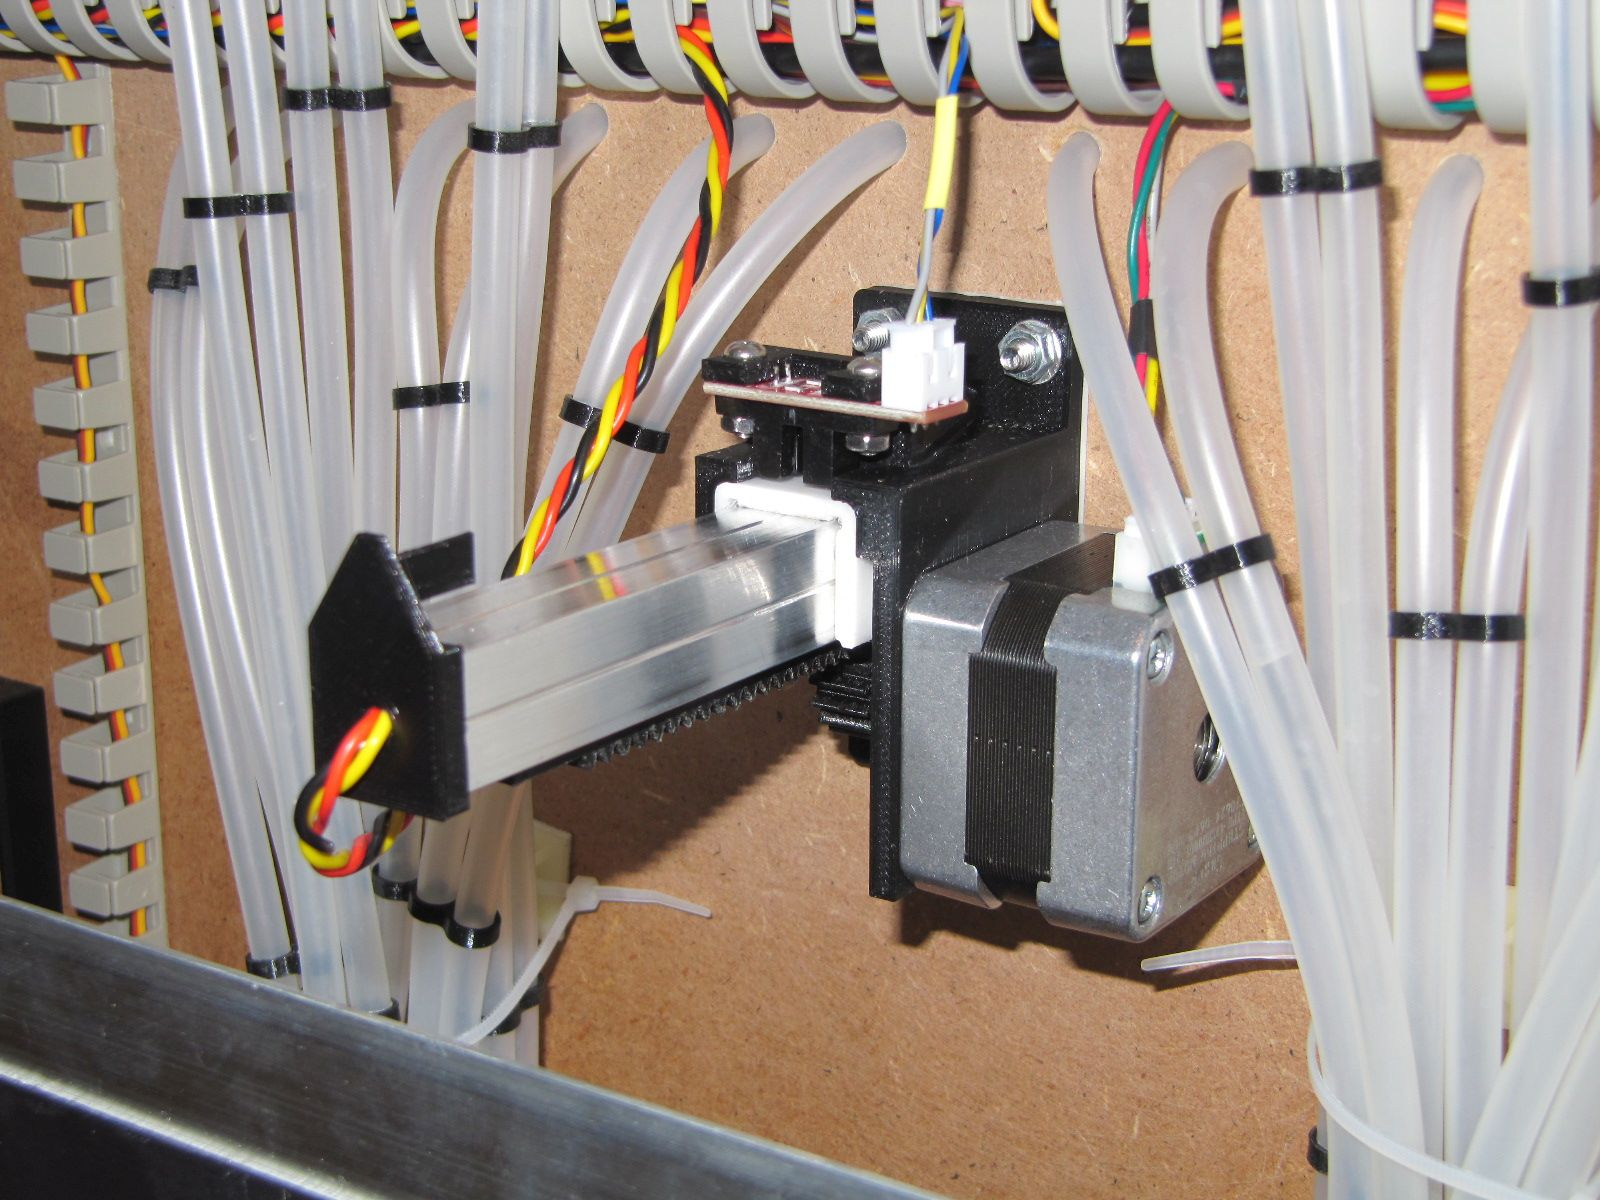
\includegraphics[height=8cm]{pics/arm_rear.jpg}
  \caption{Arm Rückseite} \label{arm_rear}
\end{figure}

\begin{figure}
 \centering
 \subfigure[Arm eingefahren]{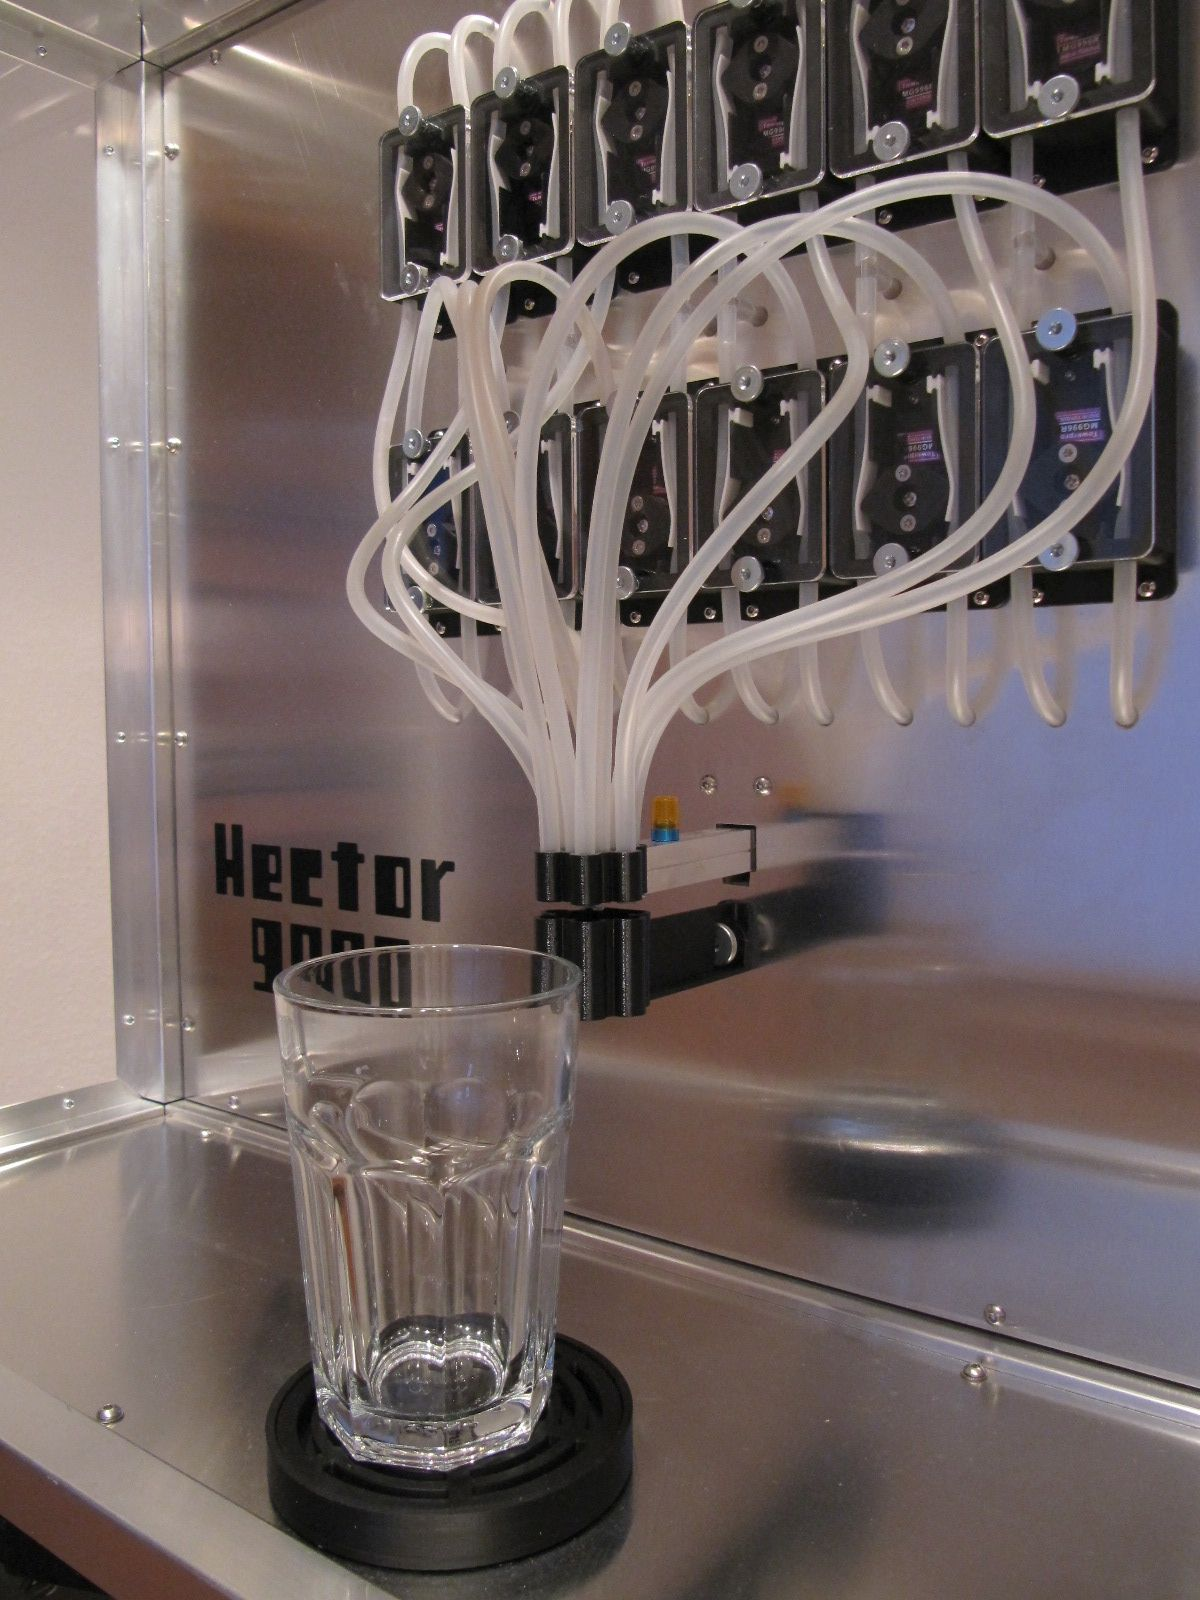
\includegraphics[height=8cm]{pics/arm_front_in.jpg}}
 \subfigure[Arm ausgefahren]{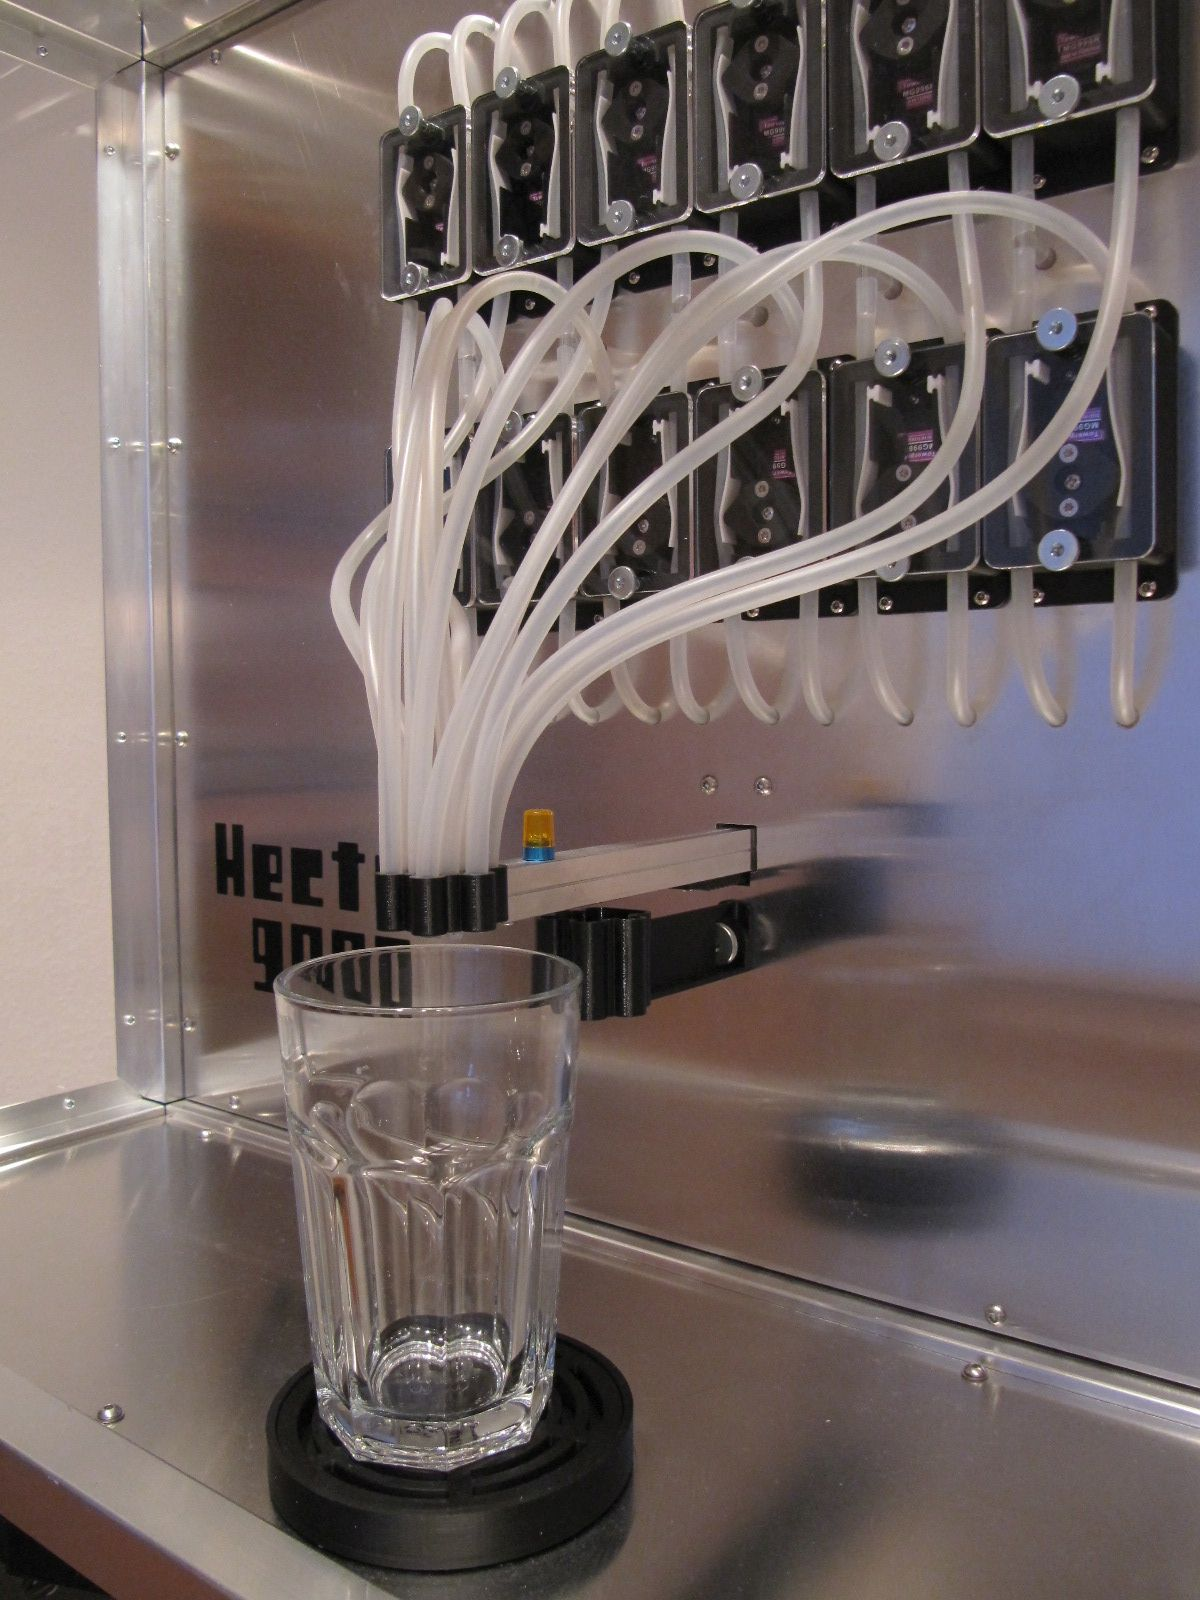
\includegraphics[height=8cm]{pics/arm_front_out.jpg}}
 \caption{Endpositionen des Arms} \label{arm_front_in}
\end{figure}

\begin{figure}
  \centering
  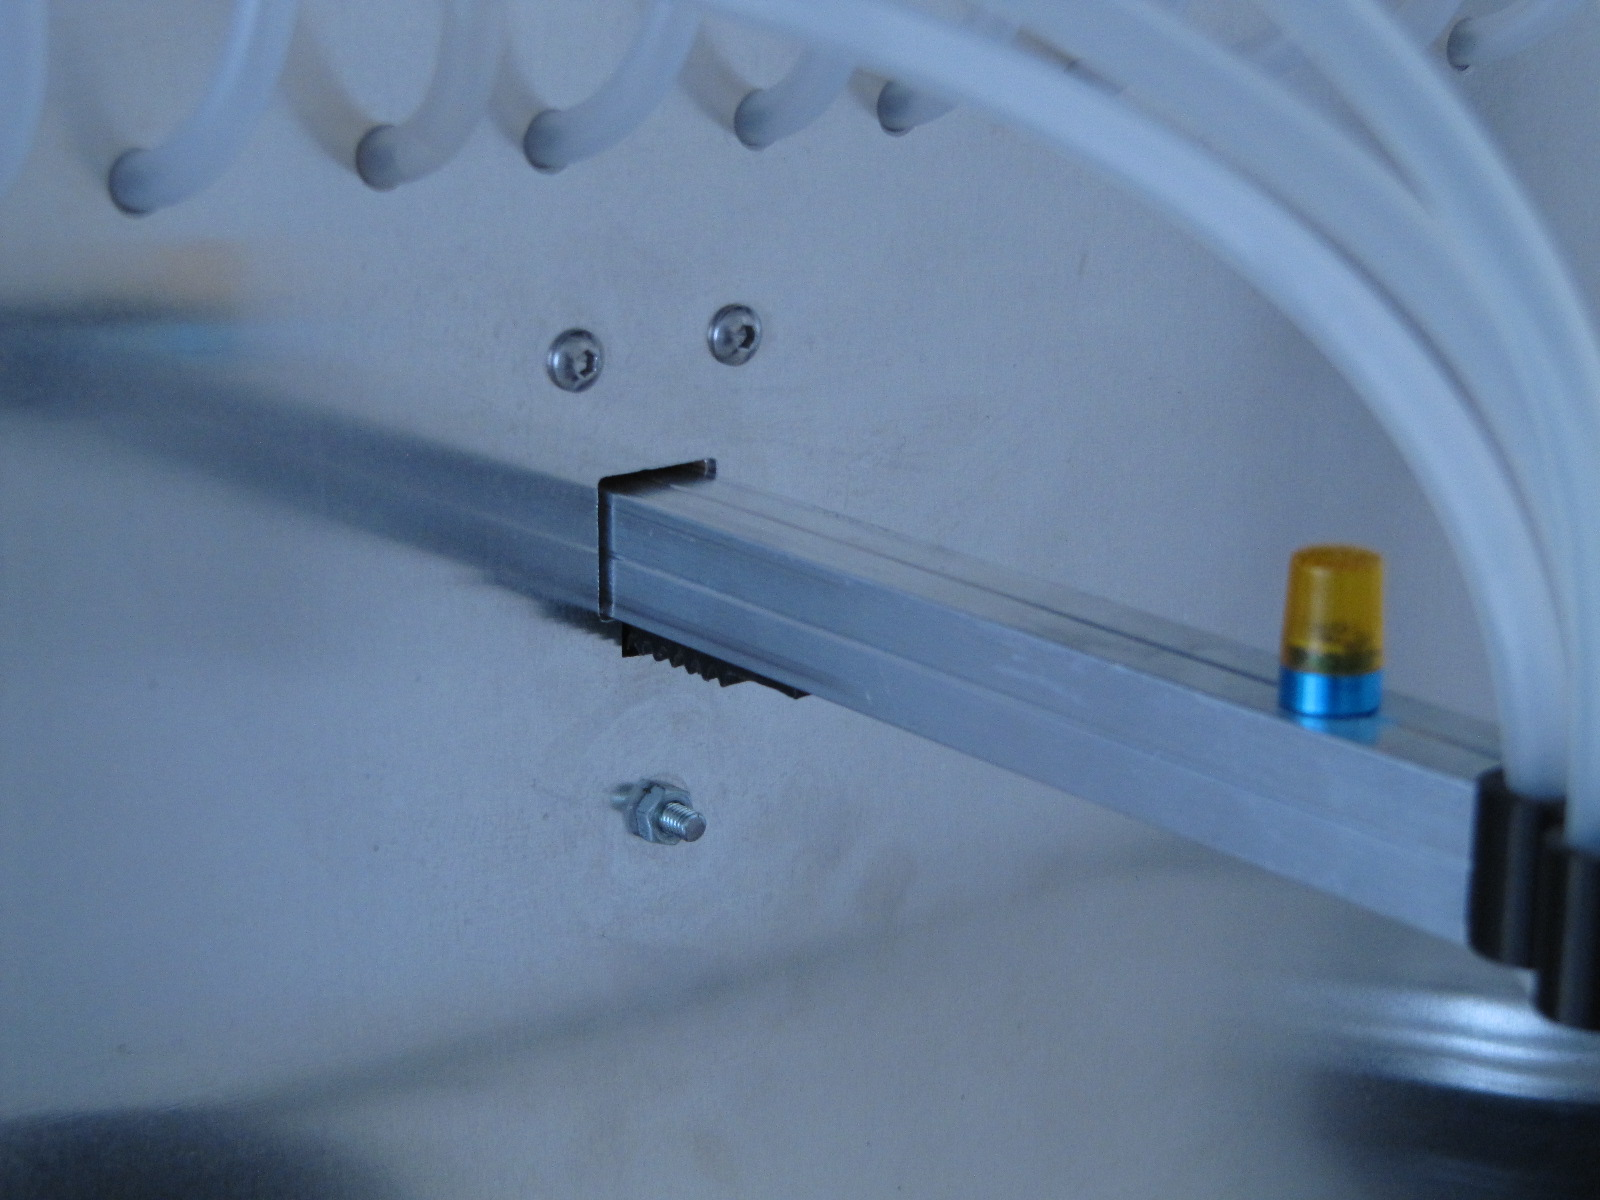
\includegraphics[height=8cm]{pics/nodrip.jpg}
  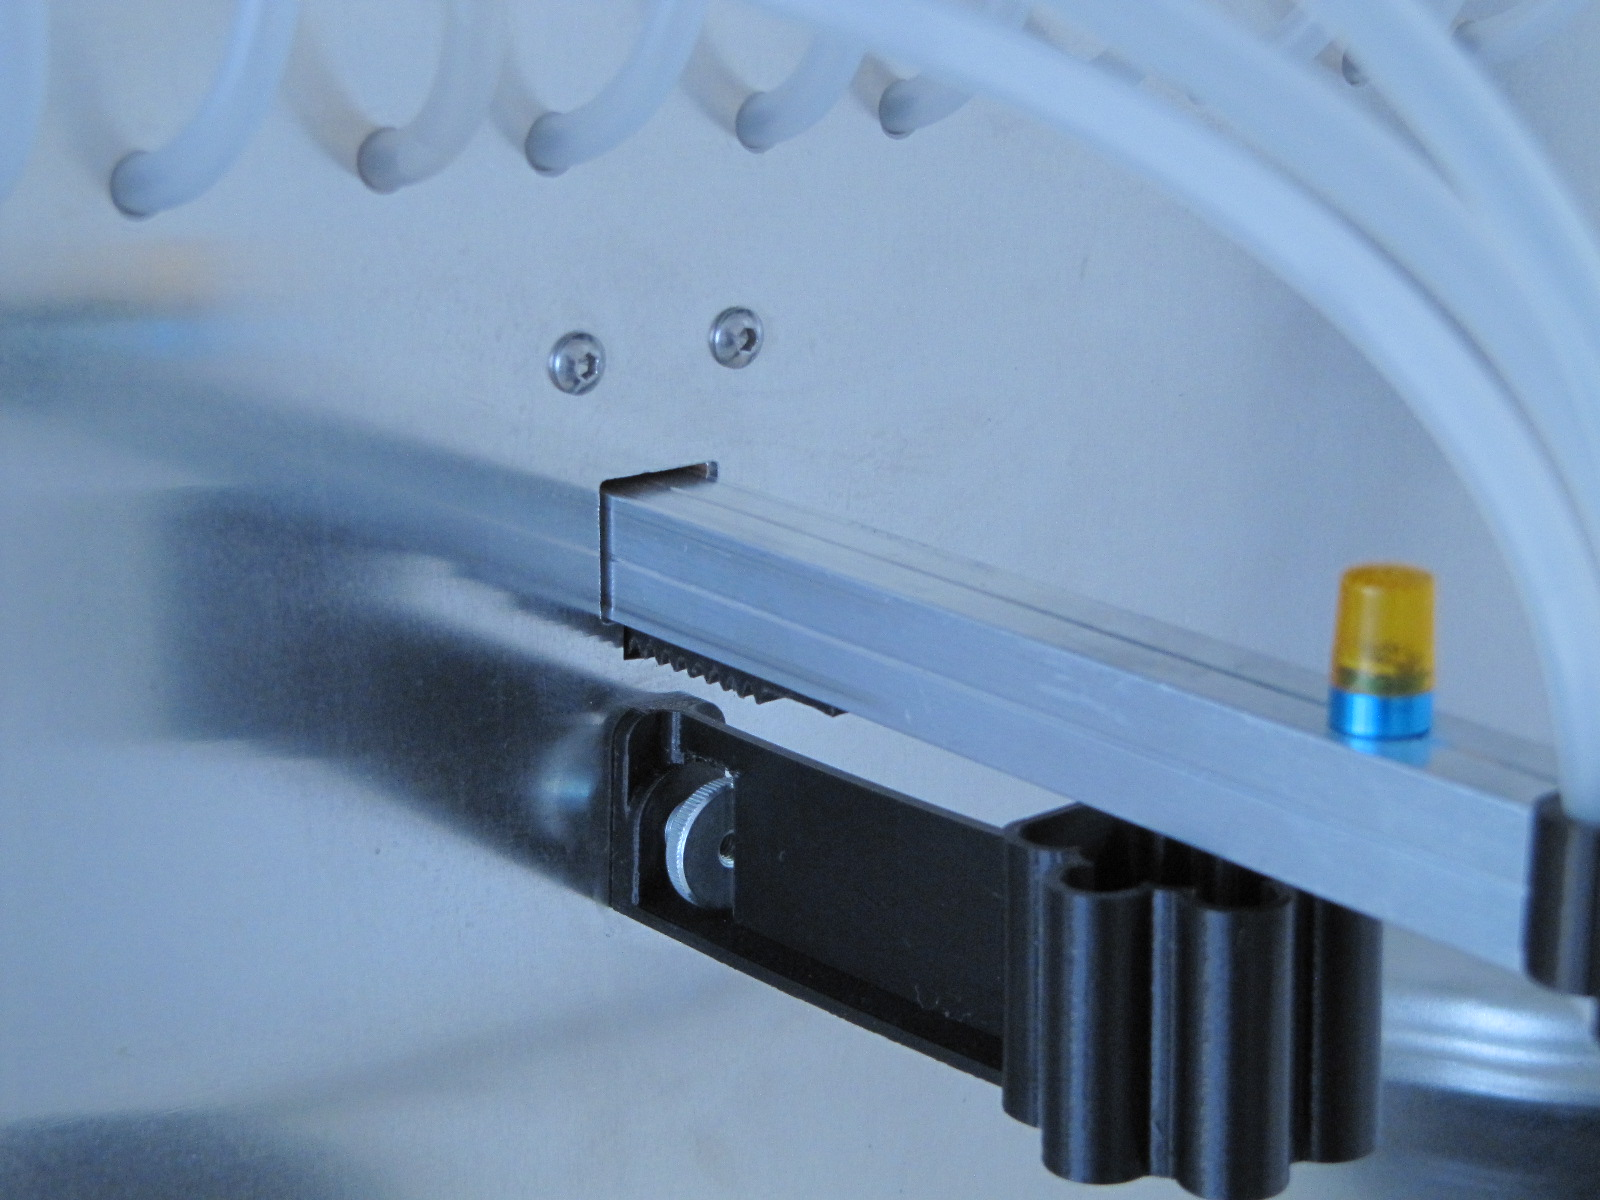
\includegraphics[height=8cm]{pics/yodrip.jpg}
  \caption{Montage des Tropfenfängers} \label{drip}
\end{figure}

\subsubsection{Glocke}
Bei dem Nachbau der Mechanik für die Glocke ist darauf zu achten, dass der Mittelpunkt der Glocke \SI{100}{\milli\metre} von der Drehachse des Arms entfernt ist. Zur Befestigung der Glocke ist eine Halterung vorgesehen (Abb. \ref{bell_mount}). Um die notwendigen Löcher in die Glocke zu bohren, wird die Halterung als Bohrlehre benutzt. Die Montage des Fingers an der Rückwand ist eigentlich selbsterklärend. Zur Befestigung der Motorhalterung (Bell\_servo-bracket.stl) an der Rückwand ist es ratsam, Einschlagmuttern oder Gewindeeinsätze zu verwenden, so kann der Finger später leicht justiert werden (Abb. \ref{finger}).

\begin{figure}
  \centering
  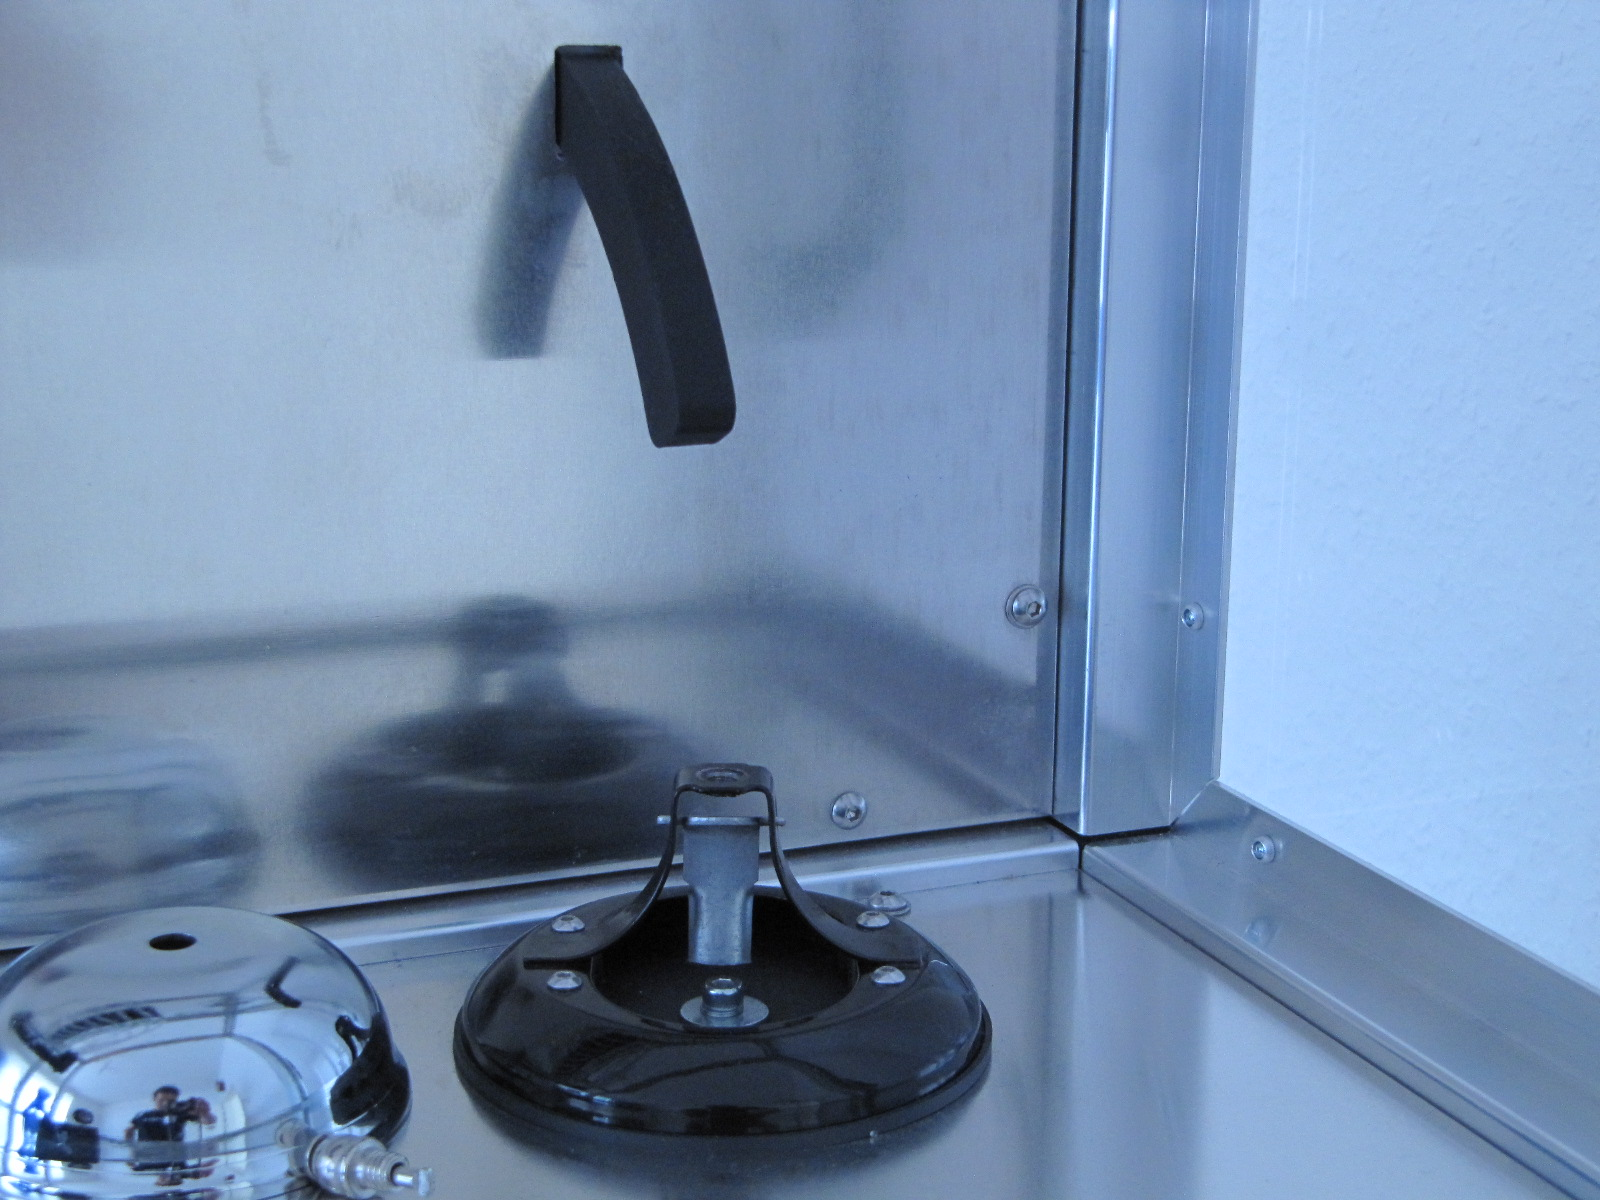
\includegraphics[height=8cm]{pics/bell_mount.JPG}
  \caption{Befestigung der Glocke} \label{bell_mount}
\end{figure}

\begin{figure}
  \centering
  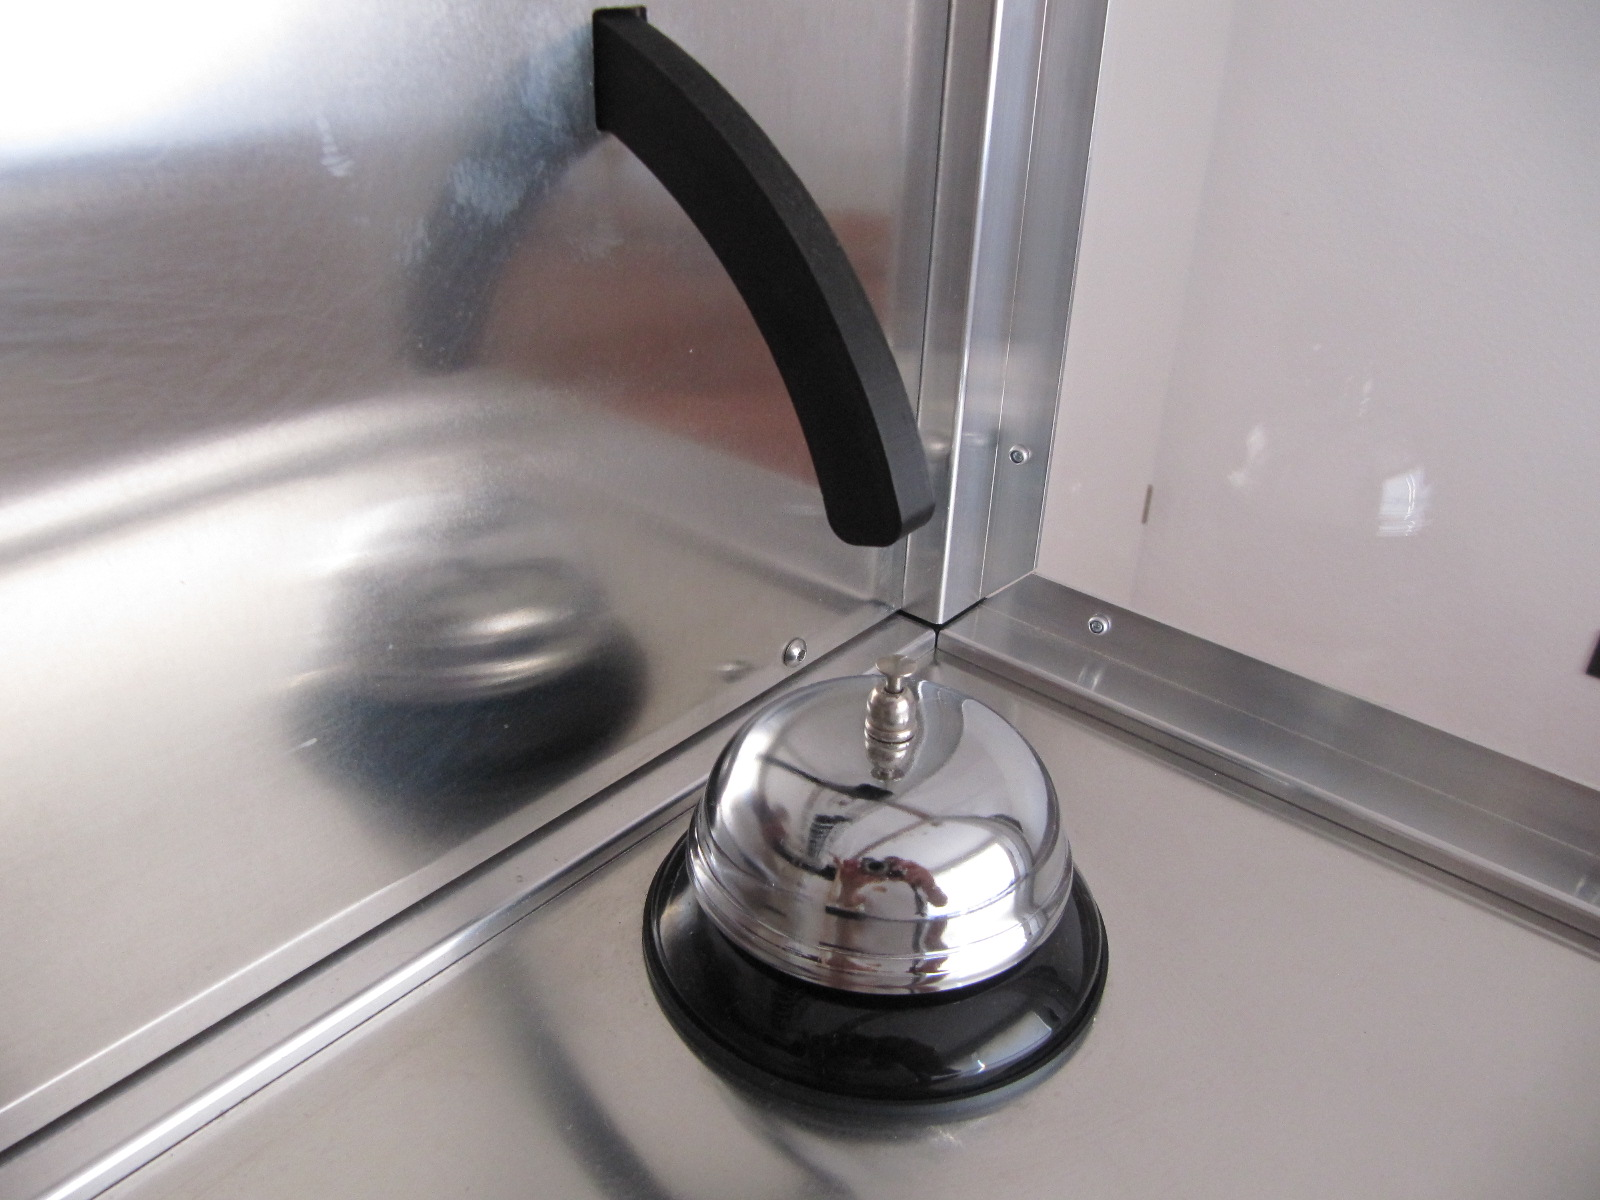
\includegraphics[height=8cm]{pics/bell.JPG}
  \caption{Glocke} \label{bell}
\end{figure}

\begin{figure}
  \centering
  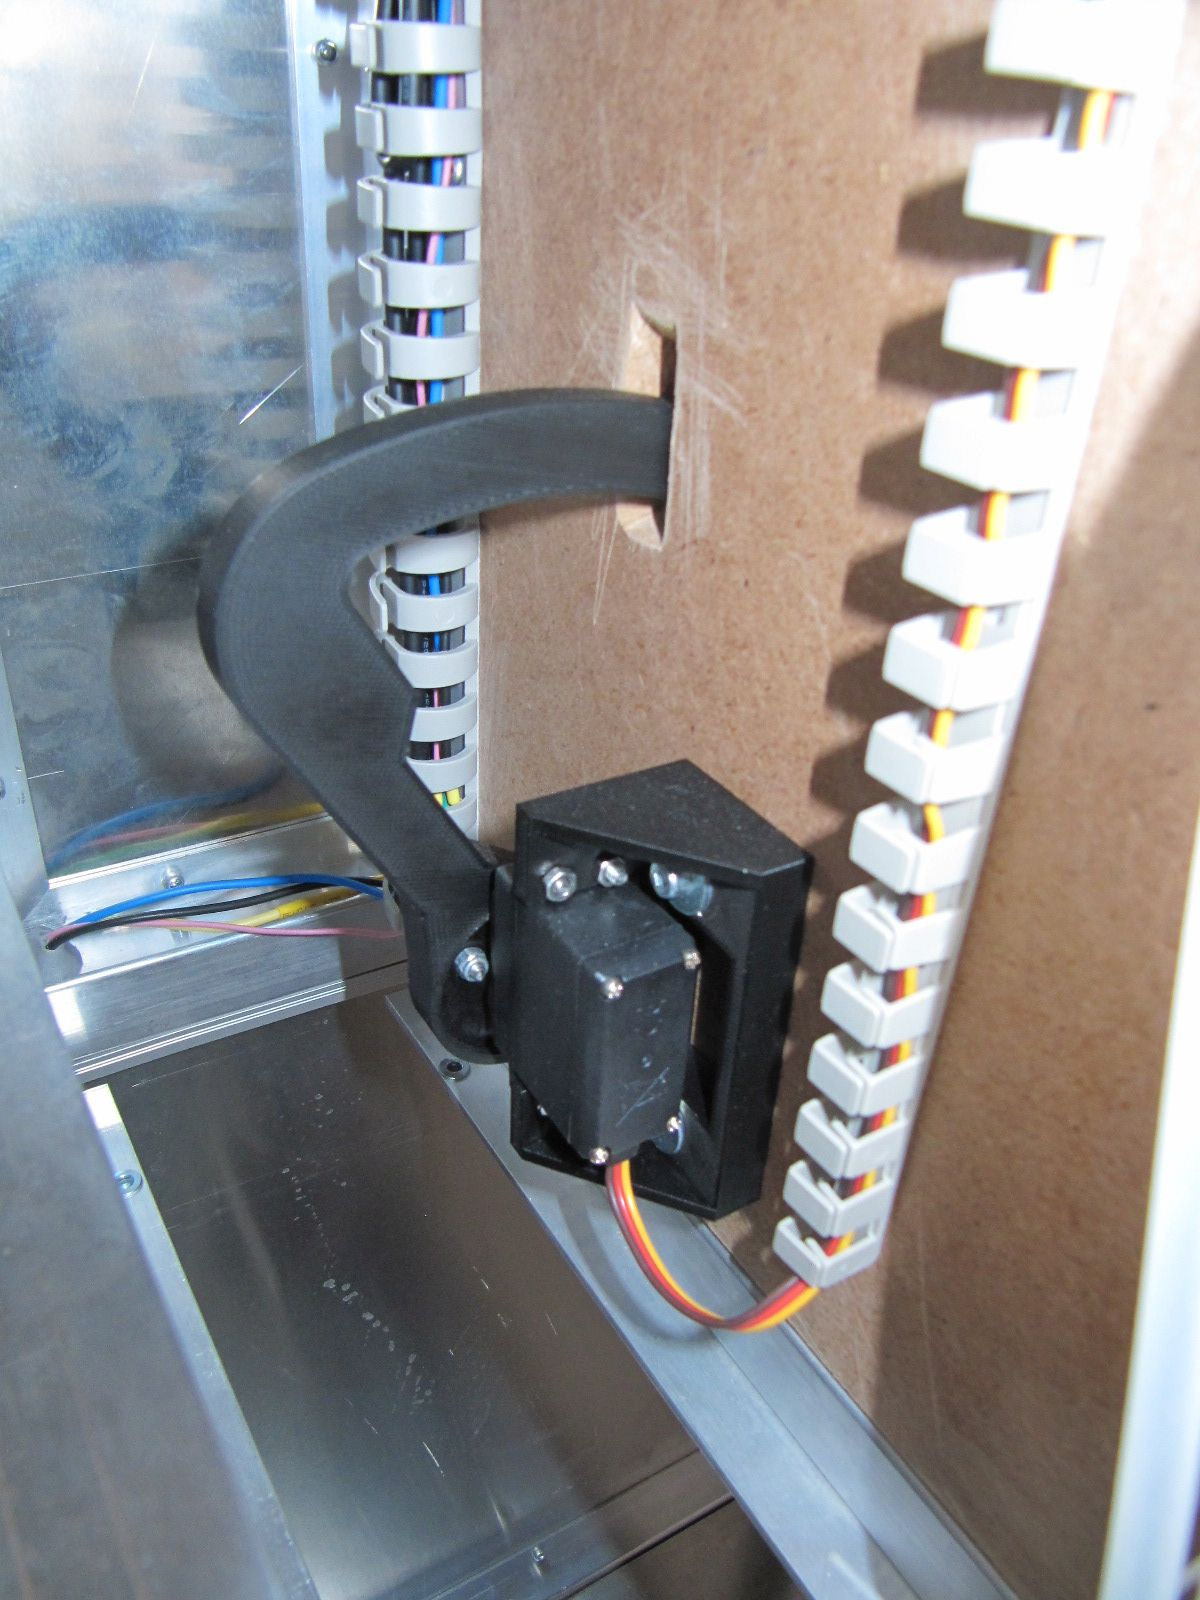
\includegraphics[height=8cm]{pics/finger.JPG}
  \caption{Finger mit Halterung} \label{finger}
\end{figure}

\subsubsection{Schläuche}
Um Flüssigkeiten und Luft zu transportieren, werden Silikonschläuche mit \SI{6}{\milli\metre} Außendurchmesser und \SI{4}{\milli\metre} Innendurchmesser verwendet. Es muss auf jeden Fall darauf geachtet werden, dass die Schläuche für den Einsatz mit Lebensmitteln vorgesehen sind. Um die Schläuche durch das Gehäuse, die Ventile und den Dosierkopf zu führen, hat es sich bewährt, ein Ende schräg abzuschneiden.
Pro Zutat werden zwei Schläuche durch ein Ventil geführt. Ein Schlauch leitet die Flüssigkeiten von der Flasche zum Dosierkopf, der andere Schlauch verbindet Luftpumpe und Flasche. Bei der Verlegung der Schläuche im Gehäuse muss darauf geachtet werden, dass sich die Schläuche nicht mit dem Arm verheddern. Wir haben dafür einfach Kabelbinder benutzt (Abb. \ref{hoses}).

\begin{figure}
  \centering
  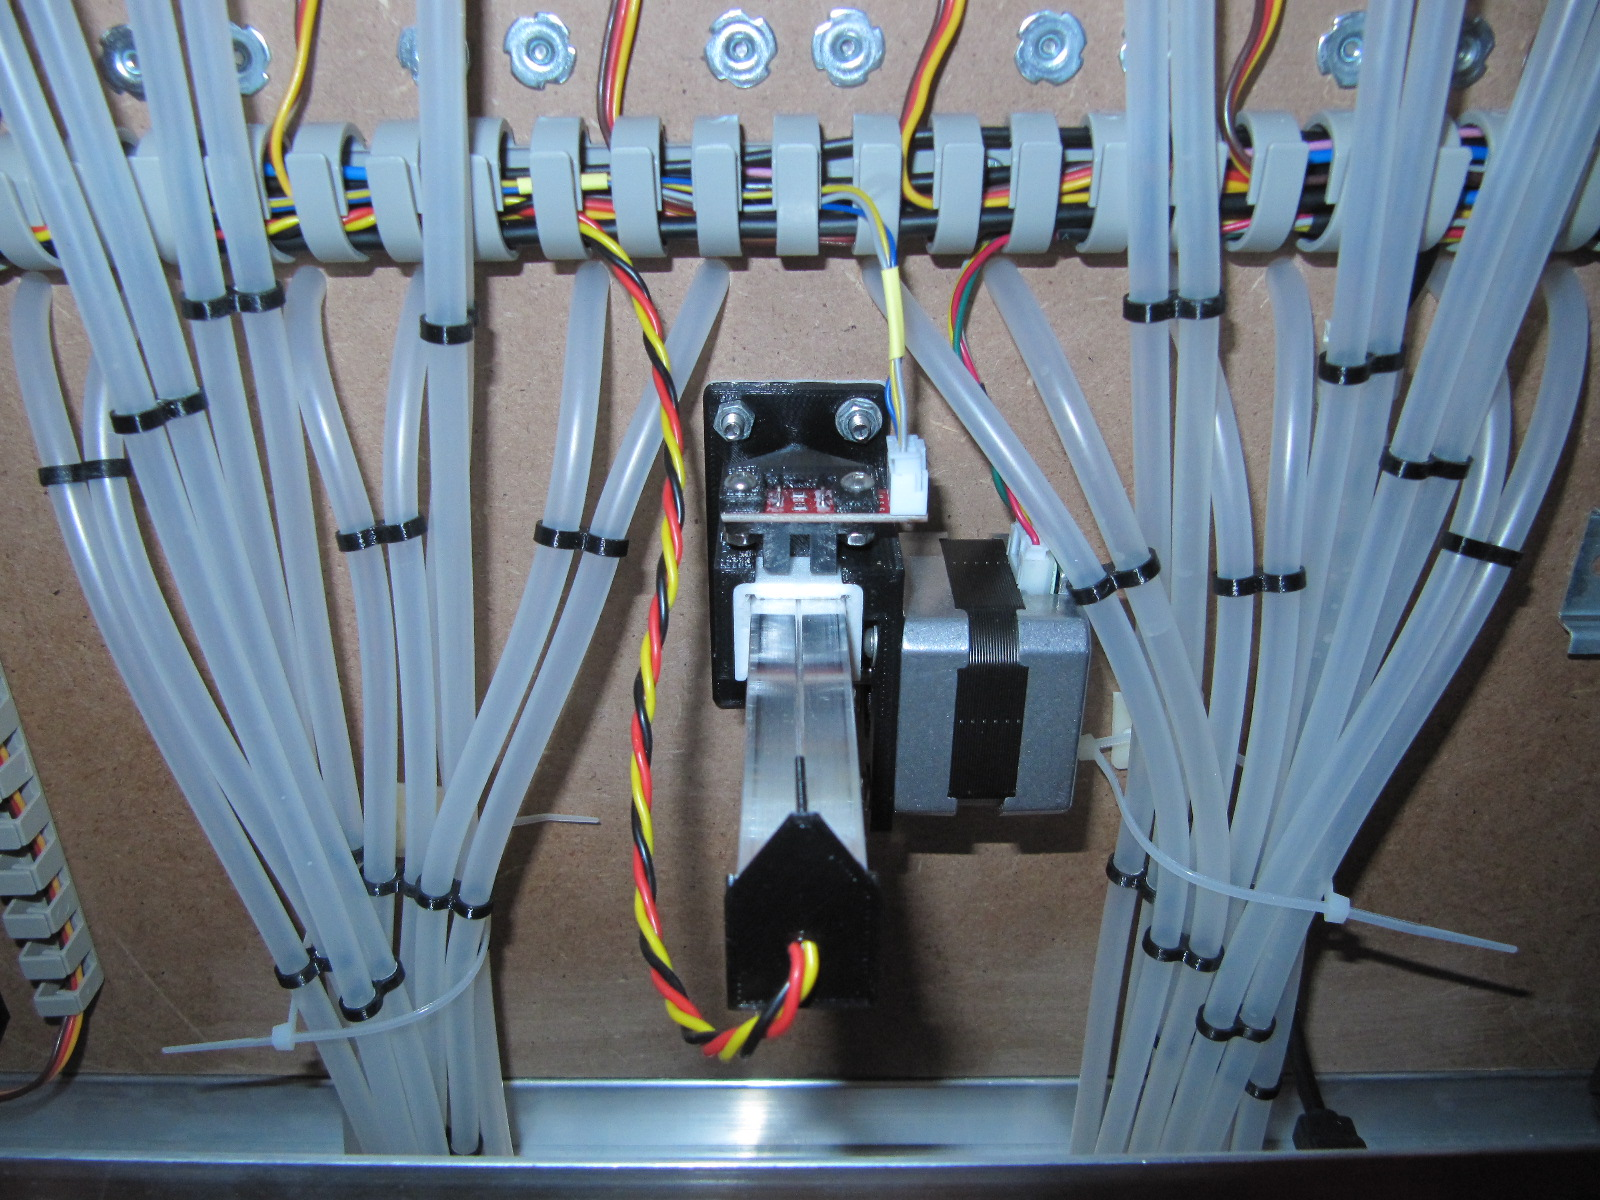
\includegraphics[height=8cm]{pics/hoses.JPG}
  \caption{Führung der Schläuche} \label{hoses}
\end{figure}

\subsubsection{Stopfen}
%\paragraph{Gummistopfen}
Die Stopfen bestehen aus einem 3D-gedruckten Kern und einer konischen Dichtung. Die Dichtung ermöglicht es, mit einer Art von Stopfen verschiedene Getränkeflaschen anzuschließen. Die Dichtungen können aus dem Gastronomiebedarf bezogen werden. Beim Druck der Kerne sollte lebensmittelechtes Filament verwendet werden. Auf einer Seite des Stopfen werden die Schläuche angeschlossen, die zu den Ventilen führen (Wichtig: Luft- und Getränkeschläuche nicht verwechseln!). Auf der anderen Seite des Stopfens wird ein Stück Silikonschlauch angeschlossen, das bis zum Boden der Flasche reicht.

\begin{figure}
  \centering
  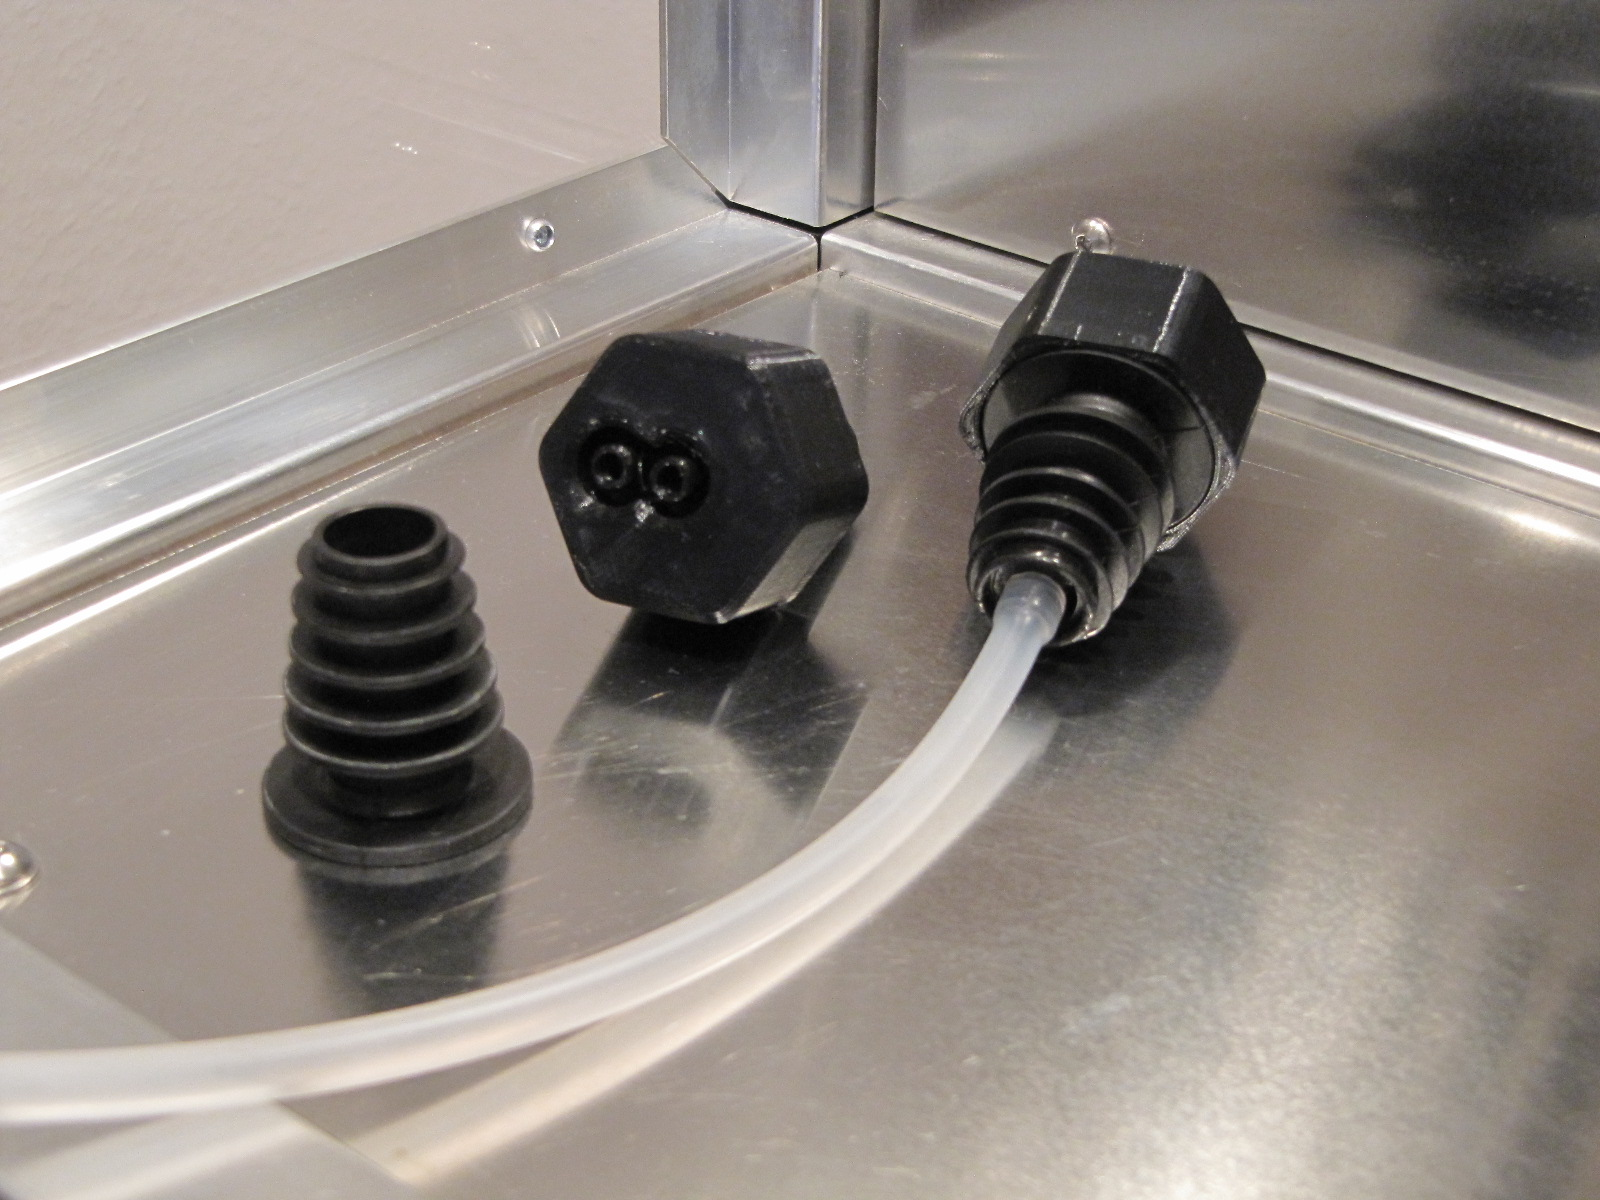
\includegraphics[height=8cm]{pics/plugs}
  \caption{Stopfen} \label{plugs}
\end{figure}

\subsubsection{Spültrichter}
Da zum Spülen der Schläuche eine Menge Wasser und Zeit notwendig ist, macht es wenig Spaß, während des Spülprogramms die ganze Zeit neben Hector zu stehen und volle Gläser auszuleeren. Wir haben deswegen einen Spültrichter konstruiert, der anstelle eines Glases auf die Waage aufgesetzt wird und das Abwasser direkt in einen Eimer oder Ausguss befördert. Der Spültrichter kann ohne Support gedruckt werden. Die Schlauchtülle ist für einen Silikonschlauch mit \SI{10}{\milli\metre} Innendurchmesser konzipiert.    
\begin{figure}
  \centering
  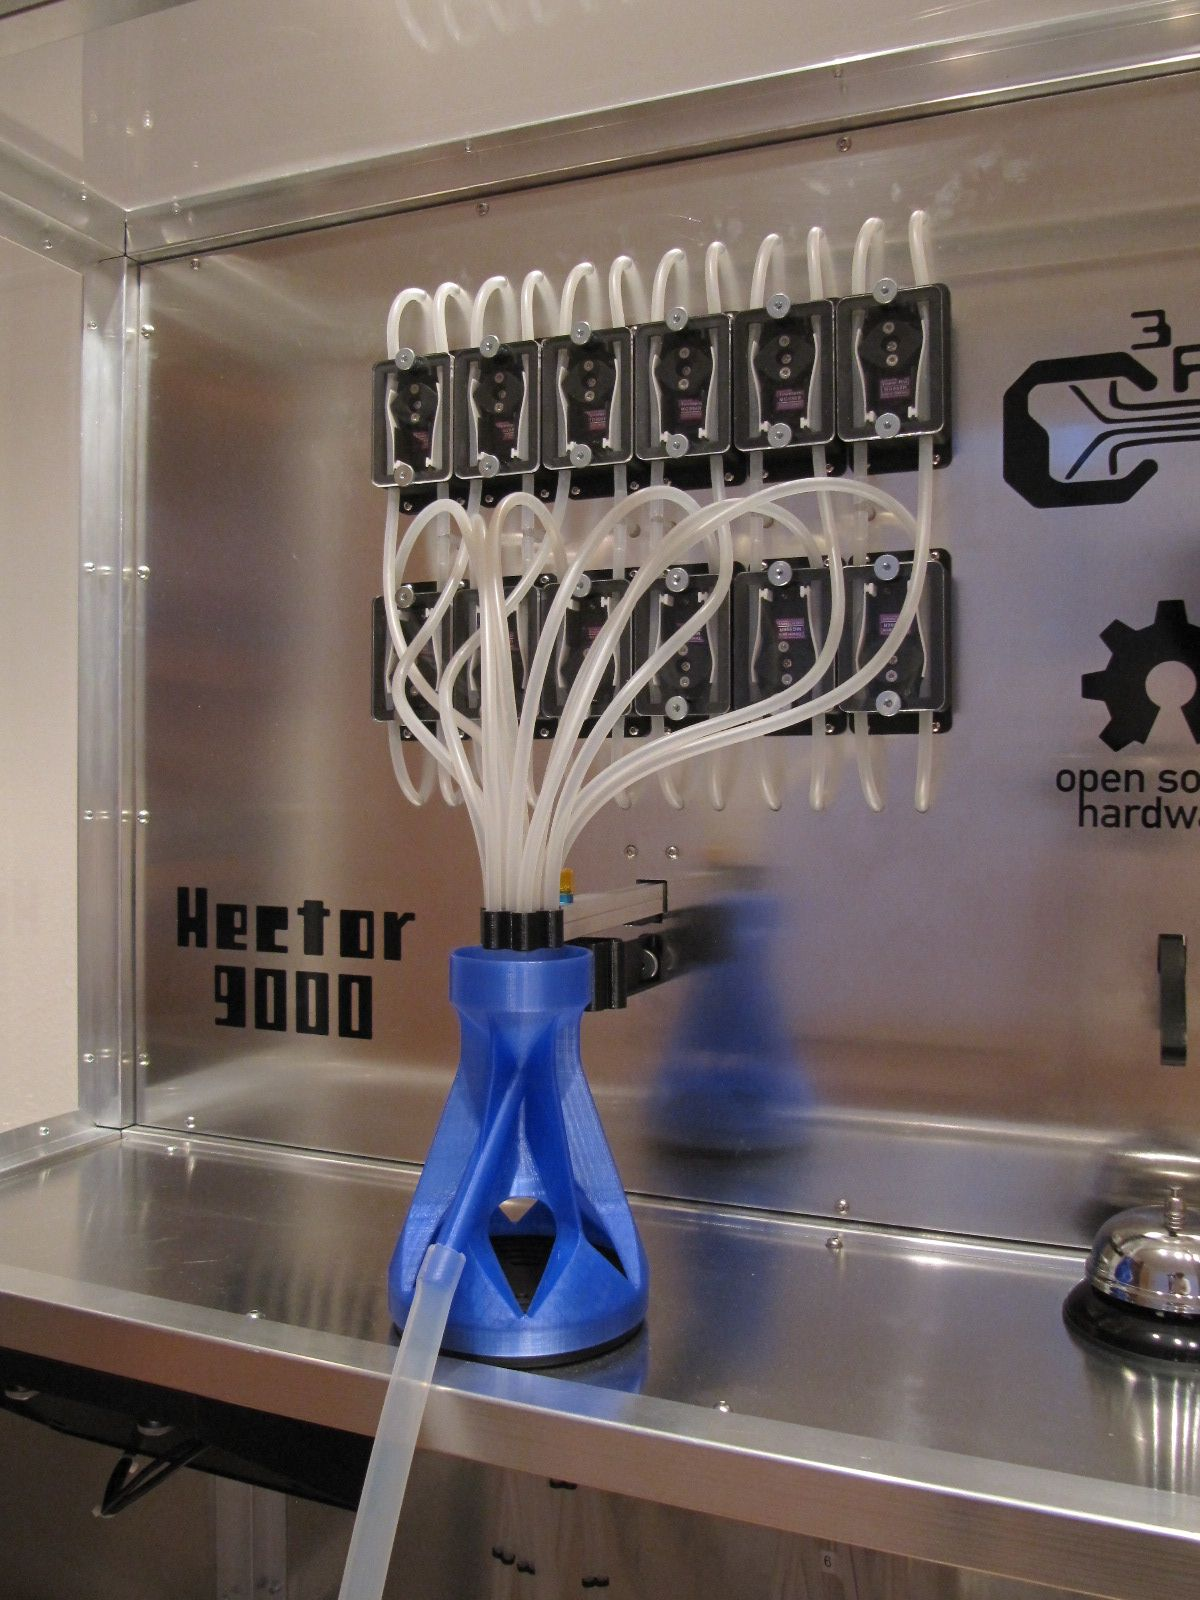
\includegraphics[height=8cm]{pics/funnel.JPG}
  \caption{Spültrichter} \label{funnel}
\end{figure}

\subsubsection{Gehäuse}
Das Gehäuse besteht aus \SI{25}{\milli\metre}-Aluminiumprofilen, die mit Aluminiumblechen und PMMA-Platten beplankt wurden. Das Blech, an dem die Waage befestigt wurde, sowie das Blech, welches die Ventile trägt, wurden zusätzlich mit einer MDF-Platte verklebt. Vor dem Verkleben wurden auf der Vorderseite der MDF-Platten Einschlagmuttern eingesetzt, um später die Hutschienen und die Pumpe zu befestigen. Die PMMA-Platten und ein Großteil der Bleche wurden mit \SI{4}{\milli\metre}-Blindnieten befestigt. Die Befestigung der Rückwand erfolgt durch M4-Schrauben. Als Gegenstück zu den Schrauben wurden in die Profile Blindnietmuttern eingesetzt. Es wird dringend empfohlen, zur Bearbeitung der Bleche und Profile spezielle Blechbohrer zu verwenden, ansonsten kann es zu Problemen beim Einsetzen der Nieten kommen. Das Gehäuse ist in der Stückliste nicht berücksichtigt, hier soll jeder seiner Kreativität freien Lauf lassen.\footnote{Außerdem haben wir keine vollständigen CAD-Daten für das Gehäuse ;)}

\begin{figure}
  \centering
  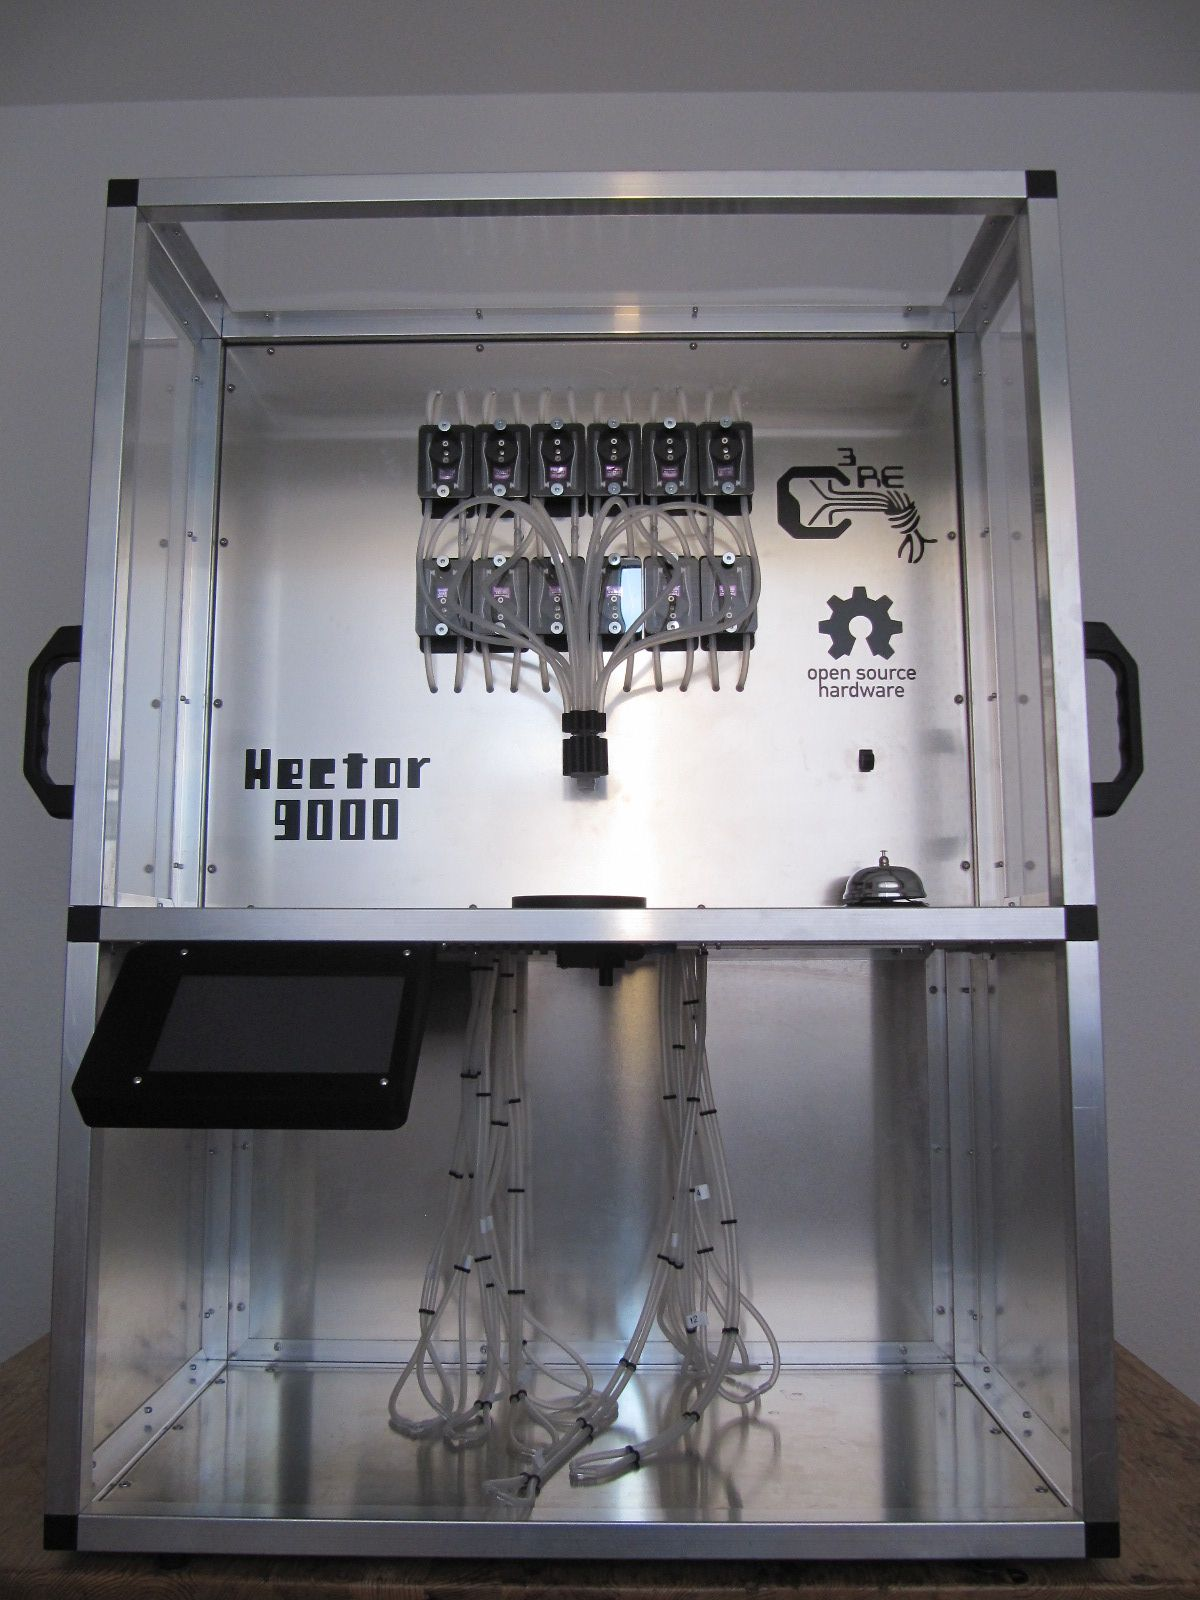
\includegraphics[height=8cm]{pics/hector9000.JPG}
  \caption{Hector 9000} \label{hector9000}
\end{figure}

\subsubsection{Display}
Zur Auswahl der Drinks haben wir uns für ein 7''-Display mit Touch-Funktion über USB entschieden. Die USB-Variante ist notwendig, da die GPIOs für andere Funktionen genutzt werden. Das Display ist an einer Querstrebe des Gehäuses befestigt. Für den Transport kann das Display in das Gehäuse gedreht werden (Abb. \ref{display_half_in}). In dem gedruckten Gehäuse für das Display sind 3 Löcher für die Montage an dem Rahmen. Für die Befestigung werden nur zwei Löcher benötigt: das mittlere Loch und ein äußeres. Das Display wird mittels Blindnietmuttern und Rändelschrauben mit dem Rahmen verschraubt. Um das Display zu drehen, wird die äußere Schraube entfernt und die mittlere Schraube gelöst. 

\begin{figure}
 \centering
 \subfigure[Display halb gedreht]{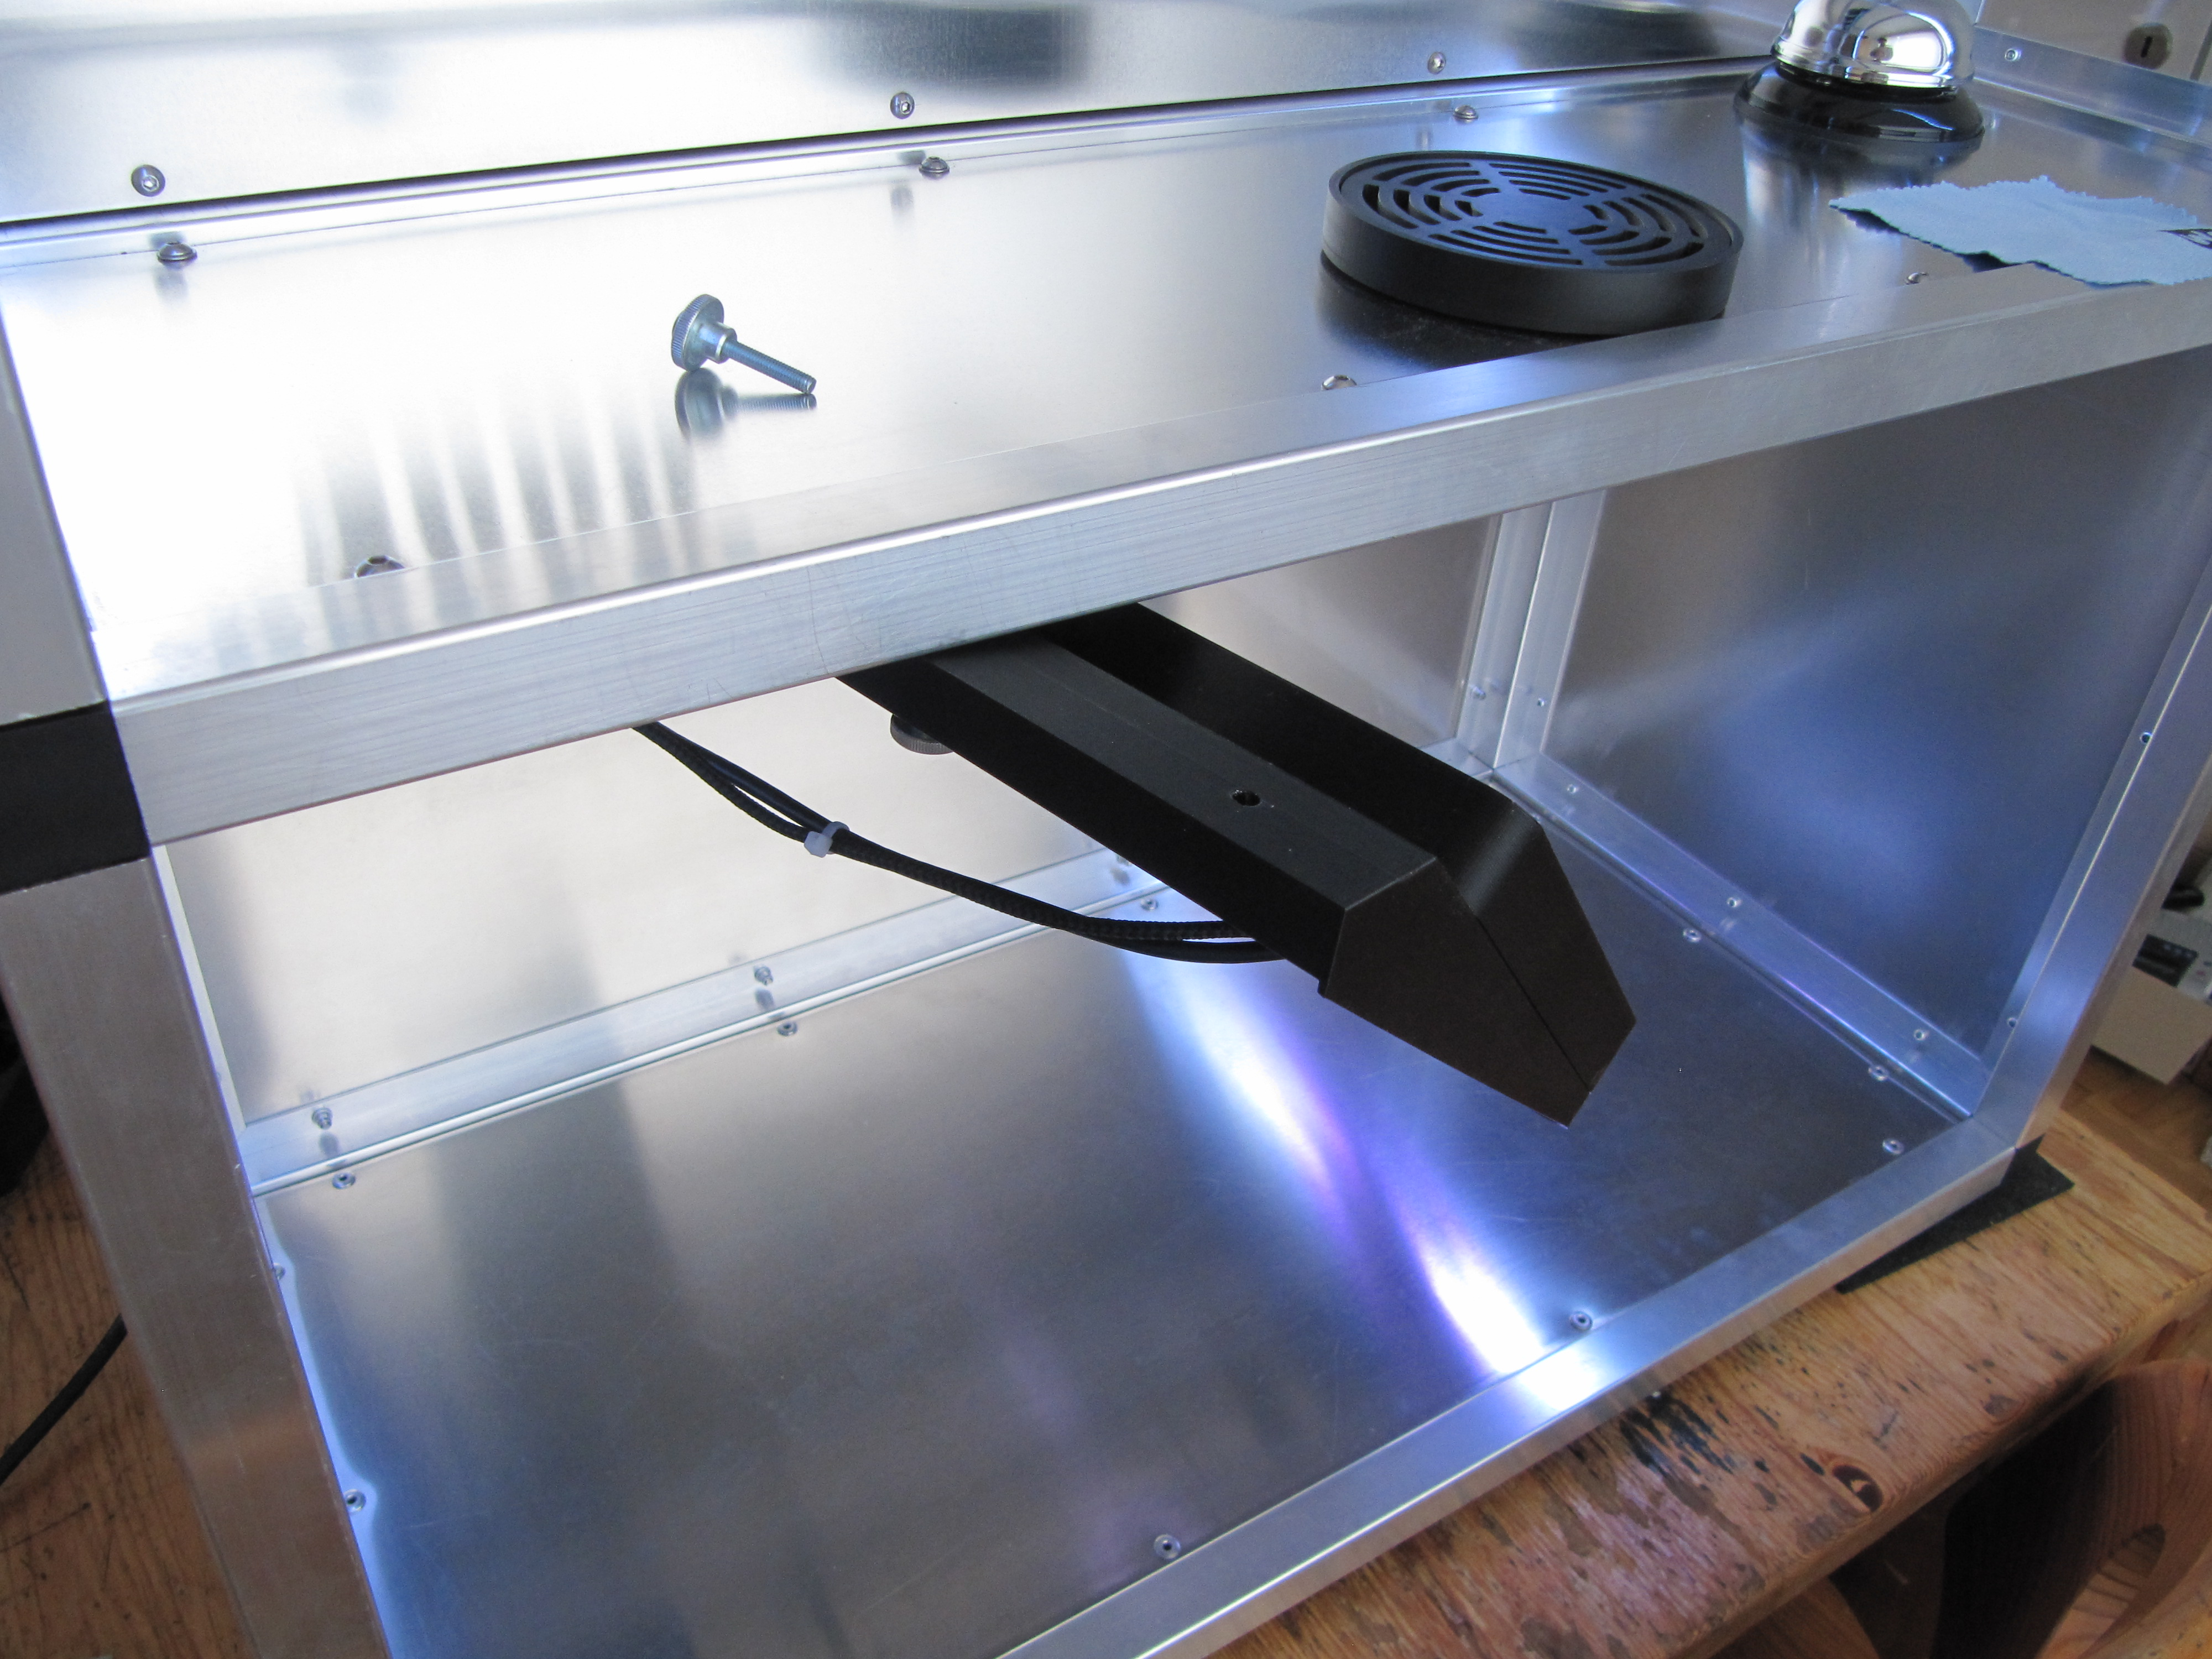
\includegraphics[height=8cm]{pics/Display_half.jpg}}
 \subfigure[Display gedreht]{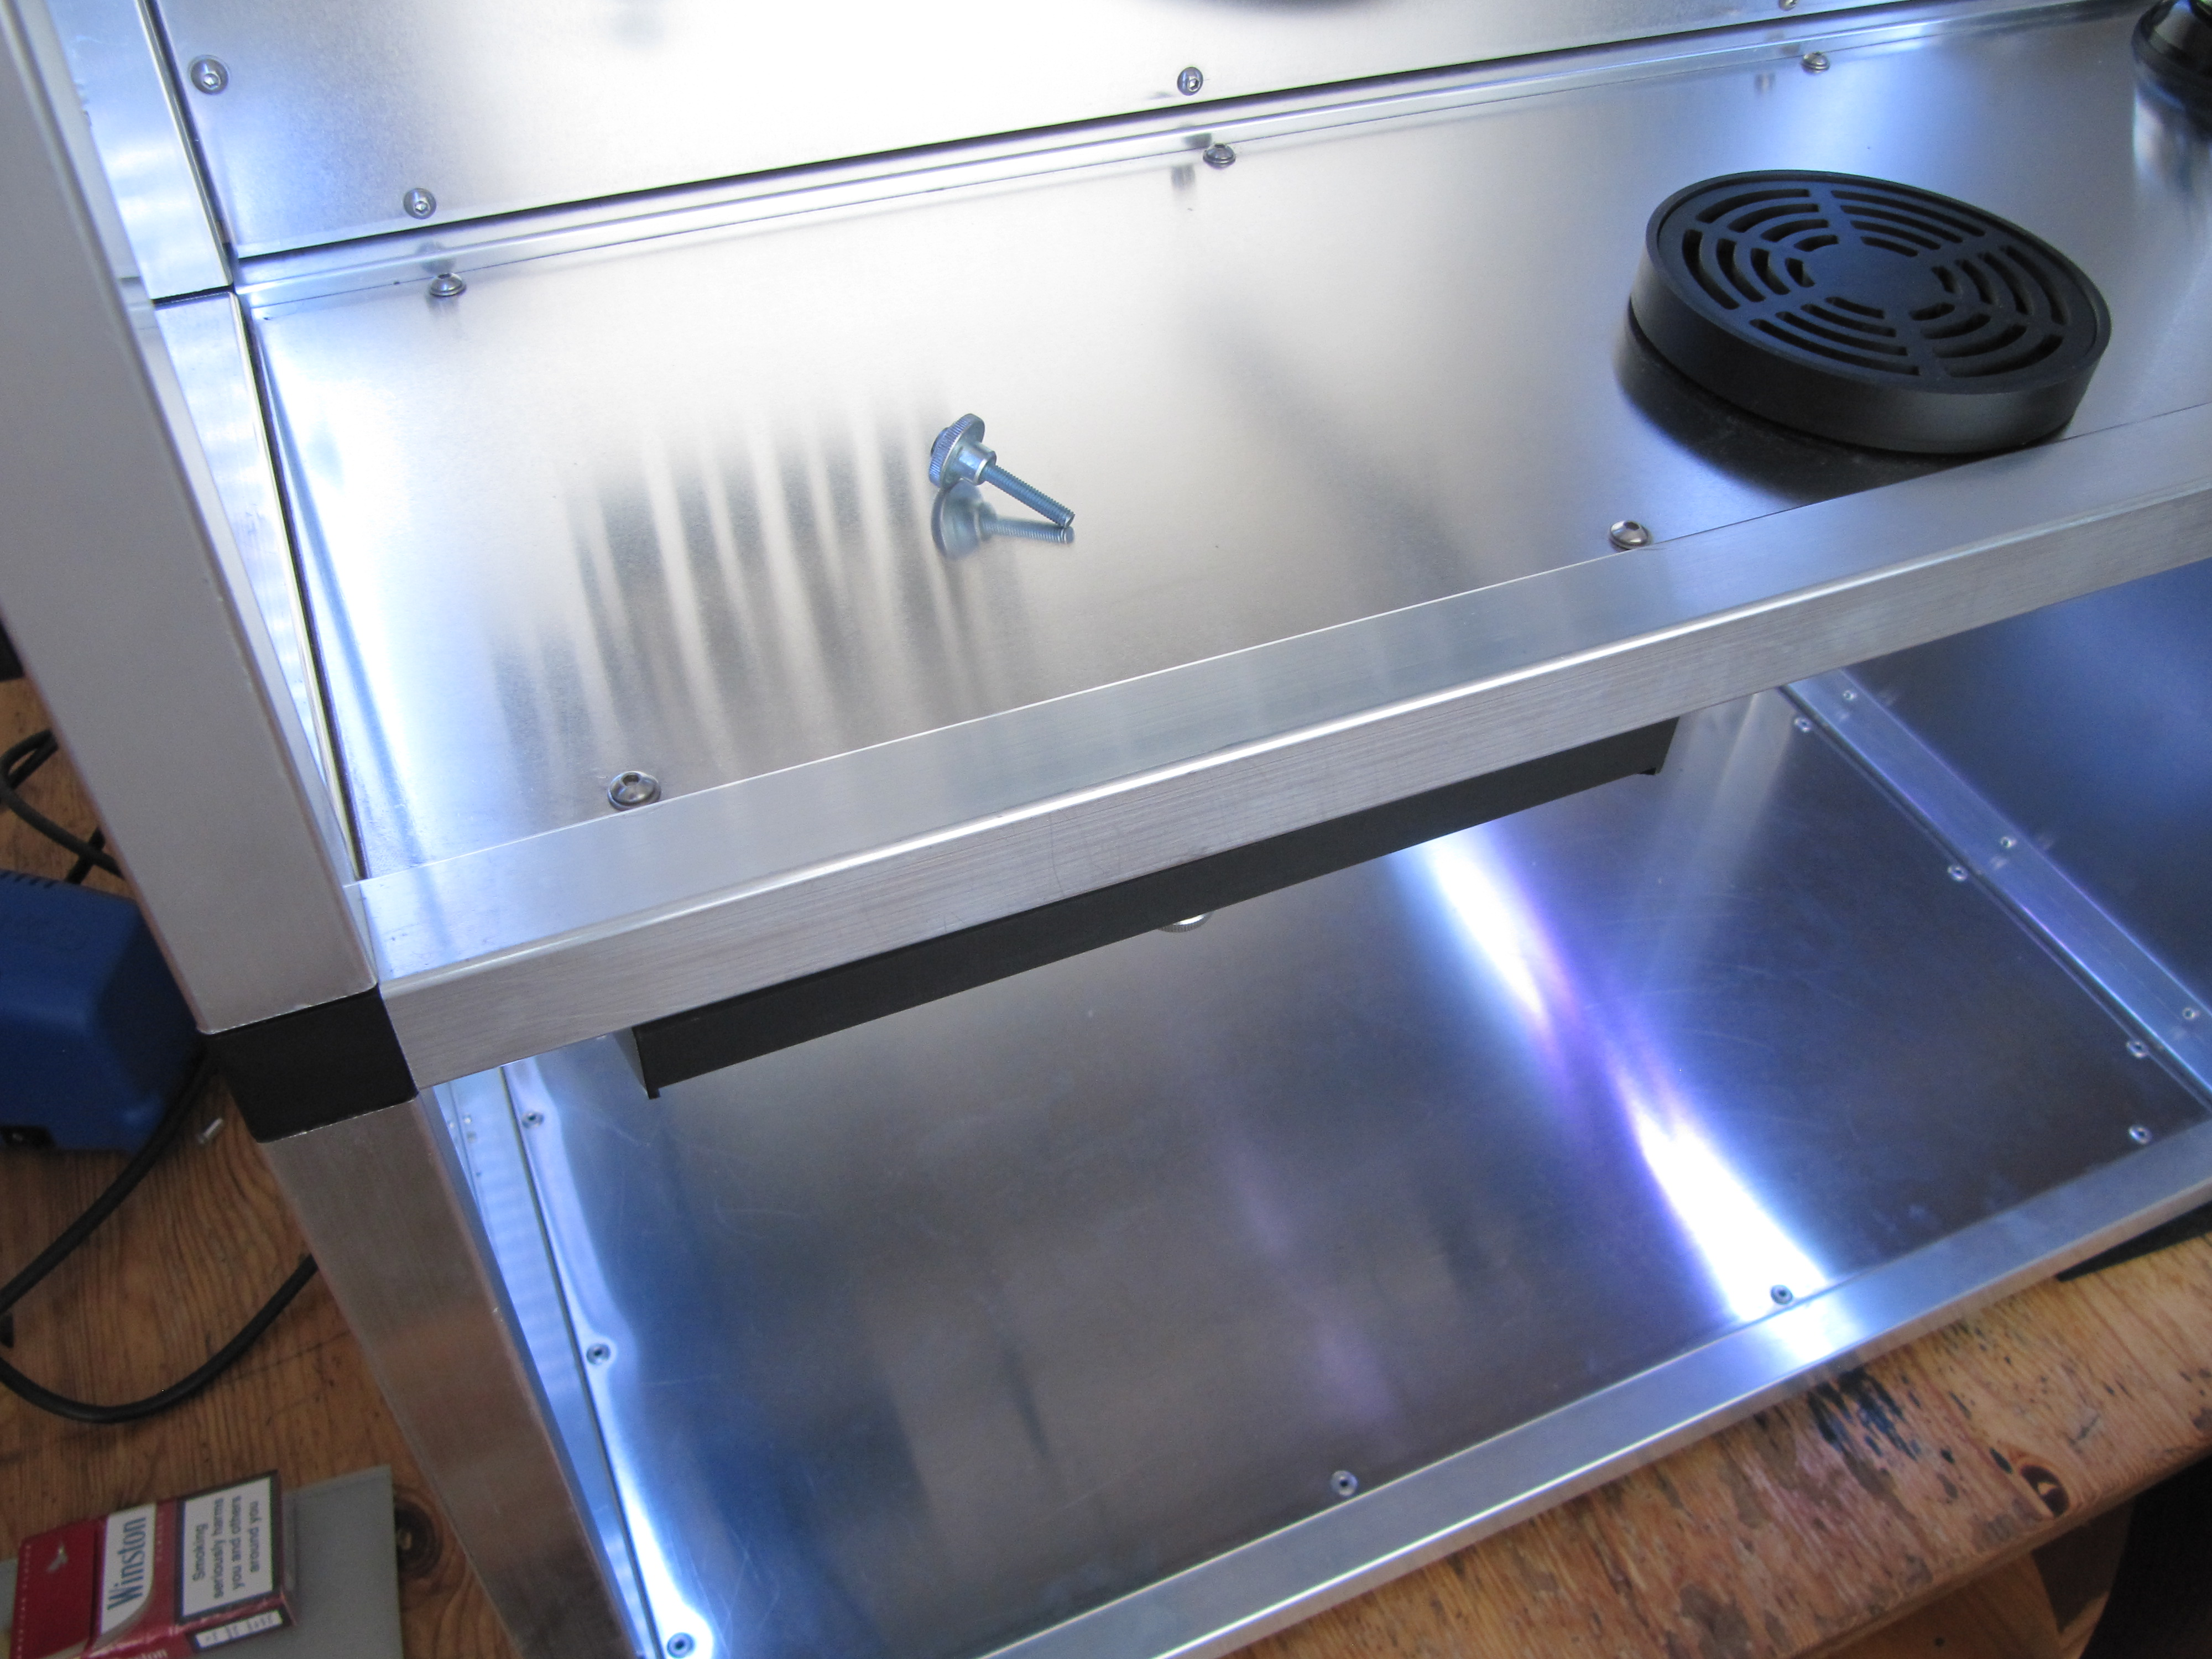
\includegraphics[height=8cm]{pics/Display_in.jpg}}
 \caption{Gedrehtes Display} \label{display_half_in}
\end{figure}

\subsection{Elektronik}

\subsubsection{Allgemeine Hinweise}
Wir haben uns entschieden, die Spannungsversorgung von Hector 9000 durch ein PC-Netzteil zu realisieren. Es ist empfehlenswert, die Spannungsausgänge des Netzteils auf Reihenklemmen zu legen und die Kabelführung in Verdrahtungskanälen vorzunehmen. Die Versorgungsspannung der LED-Streifen haben wir, ebenfalls auf Reihenklemmen, abgesichert. Außerdem lohnt es sich, die Verbindungen zwischen den Modulen durch aufgecrimpte Stecker herzustellen.    

\begin{figure}
  \centering
  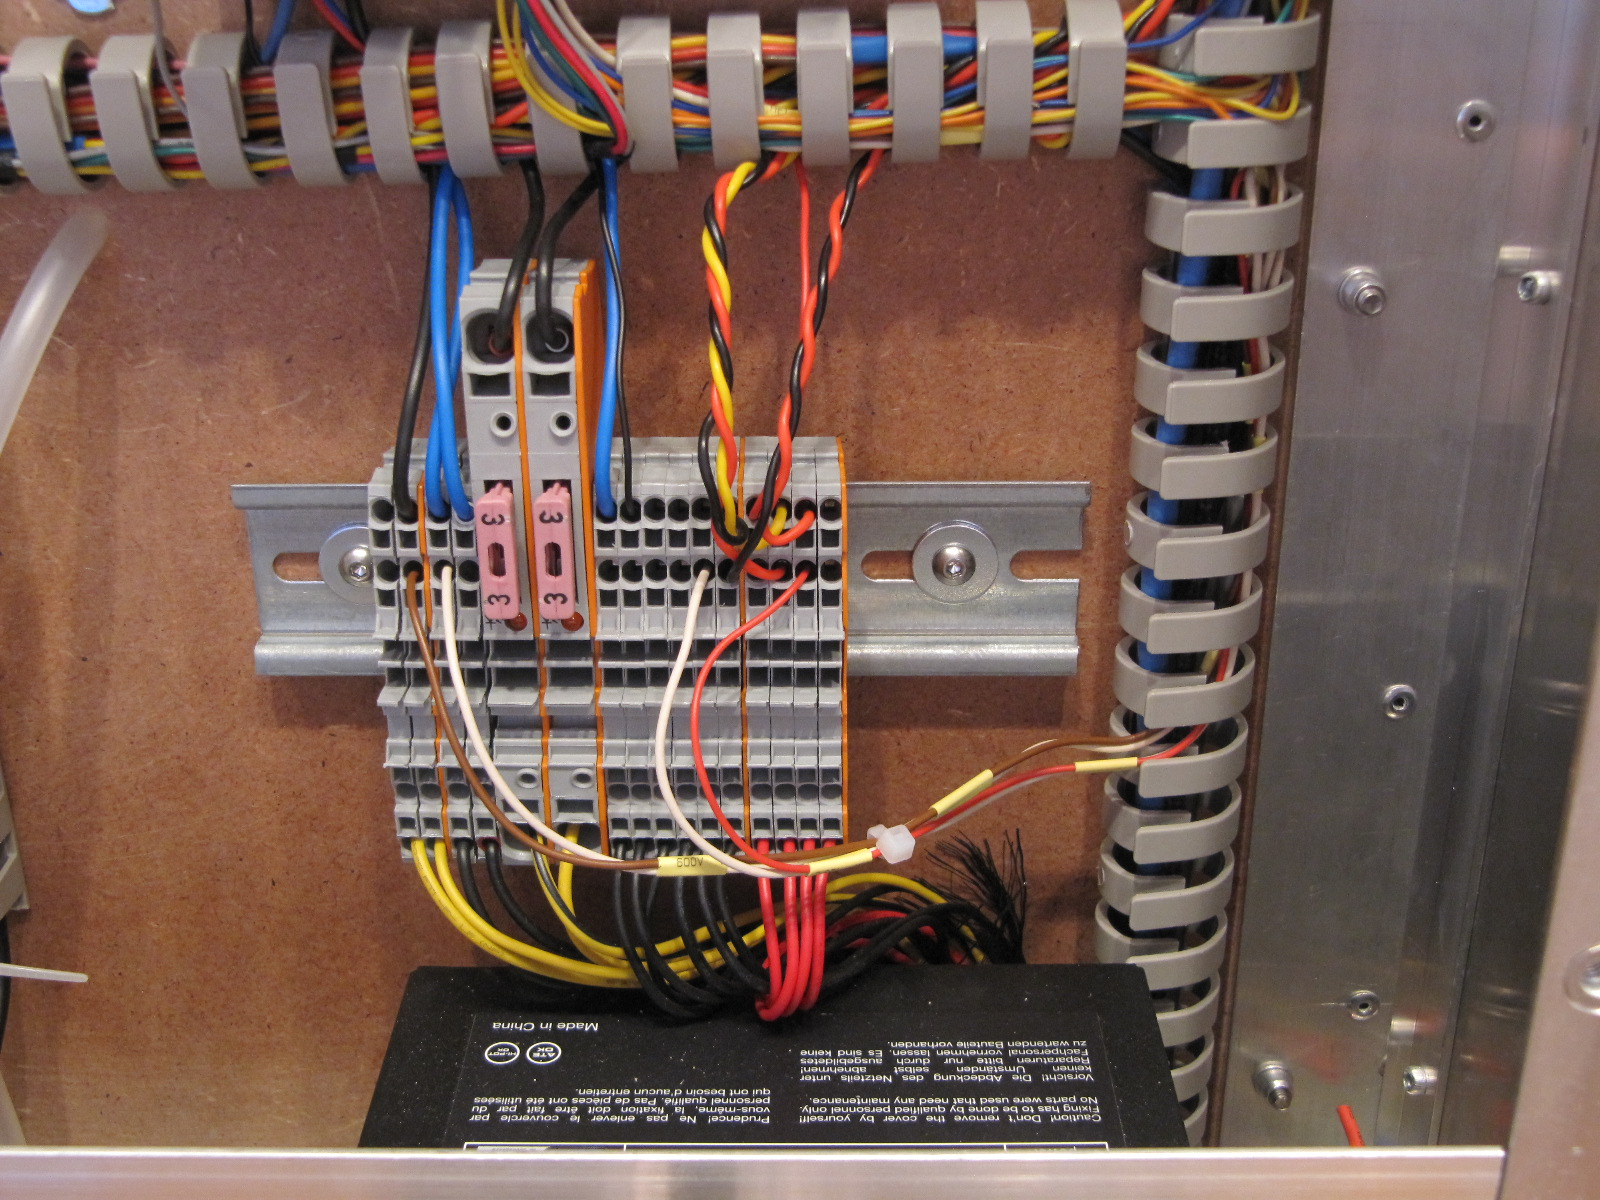
\includegraphics[height=8cm]{pics/psu}
  \caption{Spannungsversorgung} \label{psu}
\end{figure}

\begin{figure}
  \centering
  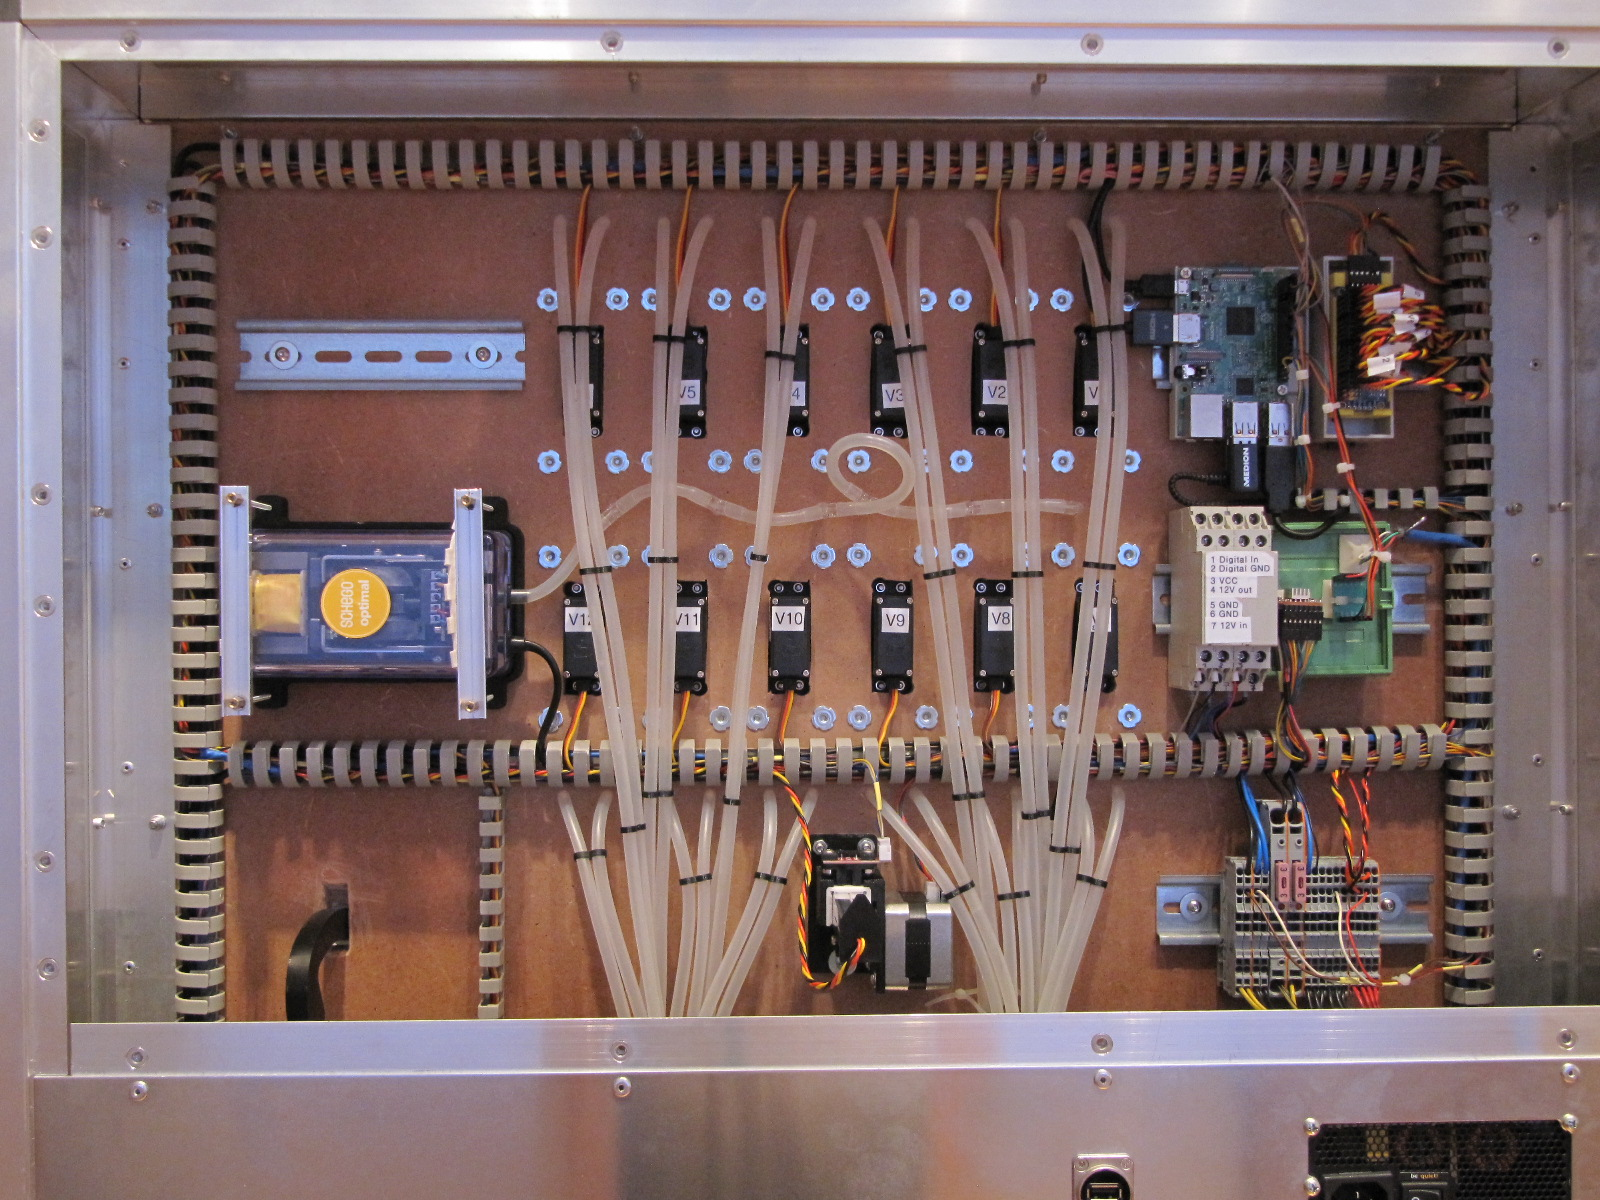
\includegraphics[height=8cm]{pics/electronic_overview}
  \caption{Geöffnete Rückseite} \label{electronic_overview}
\end{figure}

\subsubsection{Schaltung}
Die Verschaltung der einzelnen Komponenten (Abb. \ref{GPIO_overview}) ist relativ simpel. Wir empfehlen, das HX711-Board möglichst nah am Raspberry Pi zu platzieren, um die I\textsuperscript{2}C Leitungen kurz halten zu könnnen. Für die Beleuchtung wurden zwei LED-Streifen (WS2812B) parallel an einen GPIO des RPi gehängt. Pro Strang sind 15 LEDs im unteren Bereich (Getränke) und 30 LEDs im oberen Bereich des Gehäuses angeordnet. Die Pinbelegung des Raspberry Pi kann Abb. \ref{GPIO_connections} entnommen werden. Das optionale Rundumlicht muss über einen Transistor geschaltet werden (Abb. \ref{rundumlicht}).  

\begin{figure}
  \centering
  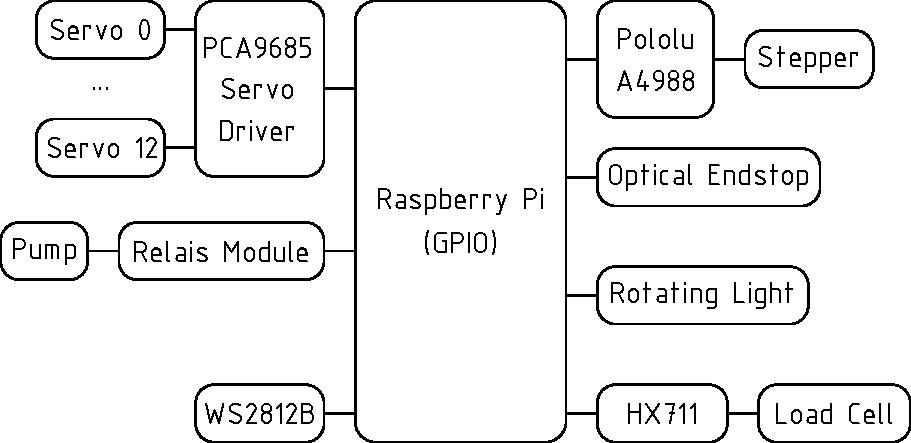
\includegraphics[height=6cm]{pics/RPi_GPIO_overview.pdf}
  \caption{Übersicht der Schaltung} \label{GPIO_overview}
\end{figure}

\begin{figure}
  \centering
  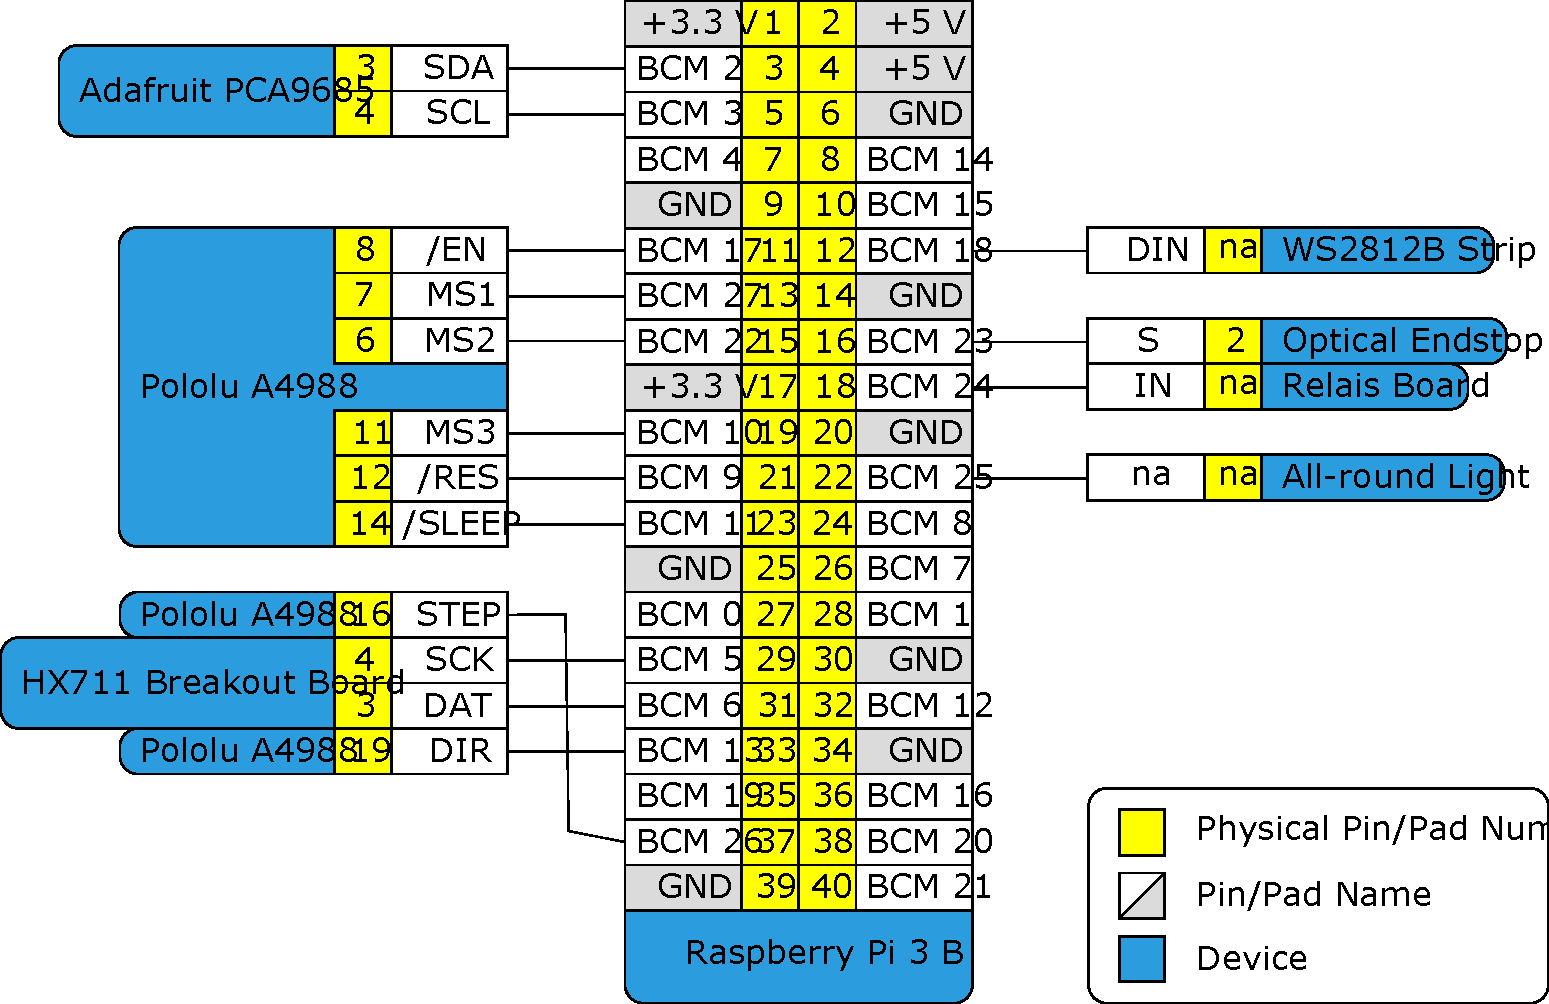
\includegraphics[height=9cm]{pics/Hector9000_connections.pdf}
  \caption{GPIO-Verbindungen} \label{GPIO_connections}
\end{figure}

\begin{figure}
  \centering
  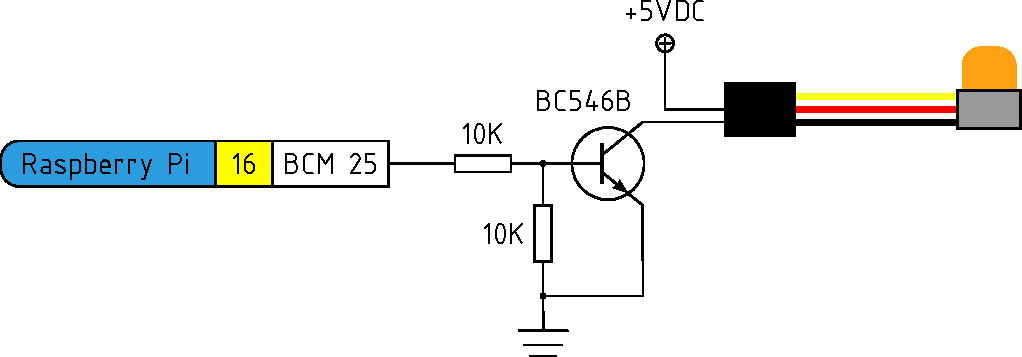
\includegraphics[height=5cm]{pics/rundumlicht.pdf}
  \caption{Anschluss des Rundumlichts} \label{rundumlicht}
\end{figure}

\FloatBarrier
\subsection{Teileliste}
In der Teileliste sind nur Komponenten aufgeführt, die zur Fertigung der einzelnen Baugruppen notwendig sind. \textbf{Kabel, Stecker, Hutschienen, Verdrahtungskanäle, \uline{Material zur Befestigung der Baugruppen im Gehäuse}, etc. müssen je nach Gehäuse individuell zusammengestellt werden.} In der Spalte \textit{Quelle} ist aufgeführt, wo wir die Teile bezogen haben. Diese Quellen sind keine Werbung für bestimmte Verkäufer oder Plattformen, sondern sollen lediglich Hinweise darauf geben, wo das Material grundsätzlich zu beziehen ist.

\begin{table}
\caption{Teileliste Waage}
\begin{tabular}{|l|l|l|l|}
\hline
Anzahl & Bezeichnung & Kommentar & Quelle\\
\hline
1 & Überlaufgitter & \texttt{Scale\_overflow\_grid.stl} & 3D-gedruckt \\
\hline 
1 & Überlaufrohr & \texttt{Scale\_overflow\_pipe.stl} & 3D-gedruckt\\
\hline 
1 & Waagschale & \texttt{Scale\_pan.stl} & 3D-gedruckt\\
\hline
1 & Abstandshalter & \texttt{Scale\_spacer.stl} & 3D-gedruckt\\
\hline
1 & Gehäuse & \texttt{Scale\_cover.stl} & 3D-gedruckt \\
\hline 
1 & Deckel & \texttt{Scale\_lid.stl} & 3D-gedruckt\\
\hline 
1 & Kabelverschraubung M10&  & eBay\\
\hline 
4 & Schraube für Thermoplaste 3x10& & Wegertseder\\
\hline
1 & Wägezelle \SI{1}{\kilo\gram} mit HX711-Board & &Amazon\\
\hline
\end{tabular}
\end{table}

\begin{table}
\caption{Teileliste Pumpe}
\begin{tabular}{|l|l|l|l|}
\hline
Anzahl & Bezeichnung & Kommentar & Quelle\\
\hline
1 & Sockel & \texttt{Schego\_830\_mount.stl} & 3D-gedruckt \\
\hline
1 & Membranpumpe Schego 830 & &Amazon\\
\hline 
2 & Streifen aus Moosgummi \SI{13}{\milli\metre} $\times$ \SI{70}{\milli\metre} & & Bastelladen \\
\hline
2 & U-Profil Aluminium \SI{13}{\milli\metre} $\times$ \SI{8}{\milli\metre} $\times$ \SI{105}{\milli\metre} & & Baumarkt\\
\hline 
4 & Gewindestange M3x65 & & Baumarkt\\
\hline
12 & DIN 934 Sechskantmutter M3 & & Wegertseder\\
\hline


\end{tabular}
\end{table}

\begin{table}
\caption{Teileliste Ventile}
\begin{tabular}{|l|l|l|l|}
\hline
Anzahl & Bezeichnung & Kommentar & Quelle\\
\hline
12 & Ventilgehäuse & \texttt{Valve\_body.stl} & 3D-gedruckt \\
\hline 
12 & Nocken & \texttt{Valve\_cam.stl} & 3D-gedruckt\\
\hline
24 & Zunge & \texttt{Valve\_tongue.stl} & 3D-gedruckt\\
\hline
12 & Deckel PMMA & \texttt{Valve\_cover.stl} & CNC/Laser \\
\hline 
12 & TowerPro MG996R Servo & nur die originalen & Hobbyking\\
\hline 
24 & DIN 965 Schraube M3x8 & & Wegertseder\\
\hline
48 & ISO 7380 Schraube M3x10 &  & Wegertseder\\
\hline
24 & DIN 933 Schraube M3x35 &  & Wegertseder\\
\hline
72 & DIN 934 Sechskantmutter M3 & & Wegertseder\\
\hline 
24 & DIN 466 Rändelmutter M3 &  & Wegertseder\\
\hline 

\end{tabular}
\end{table}

\begin{table}
\caption{Teileliste Arm}
\begin{tabular}{|l|l|l|l|}
\hline
Anzahl & Bezeichnung & Kommentar & Quelle\\
\hline
1 & Halterung & \texttt{Arm\_mount.stl} & 3D-gedruckt\\
\hline
1 & Gleiteinsatz & \texttt{Arm\_sliding\_element.stl} & 3D-gedruckt\\
\hline
1 & Zahnstange & \texttt{Arm\_rack.stl}  & 3D-gedruckt\\
\hline
1 & Ritzel & \texttt{Arm\_pinion.stl}  & 3D-gedruckt\\
\hline
1 & Auslöser & \texttt{Arm\_trigger.stl} & 3D-gedruckt\\
\hline
1 & Dosierkopf & \texttt{Arm\_pourer.stl} & 3D-gedruckt\\
\hline
1 & Tropfenfänger & \texttt{Arm\_drip\_pan.stl}  & 3D-gedruckt\\
\hline
1 & Gabellichtschranke &  & Amazon\\
\hline 
1 & Pololu A4988 & & Amazon\\
\hline 
1 & NEMA 17 Schrittmotor & & Amazon\\
\hline
1 & Alu-Vierkantprofil 15.5x15.5 & Länge ist v. Gehäuse abhängig& Baumarkt\\
\hline
1& DIN 7981 Blechschraube 2.9x6.5  & & Wegertseder\\
\hline
4 & ISO 7380 Schraube M3x6  & & Wegertseder\\
\hline
4 & ISO 7380 Schraube M3x10  & & Wegertseder\\
\hline
6 & DIN 125 Unterlegscheibe 3.2  & & Wegertseder\\
\hline
2 & DIN 934 Sechskantmutter M3 & & Wegertseder\\
\hline
3 & DIN 934 Sechskantmutter M4 & & Wegertseder\\
\hline
1 & DIN 466 Rändelmutter M4 &  & Wegertseder\\
\hline 
6 & DIN 125 Unterlegscheibe 3.2  & & Wegertseder\\
\hline
2 & Blindnietmutter M3x10 flach & & Wegertseder\\
\hline 

\end{tabular}
\end{table}

\begin{table}
\caption{Teileliste Glocke}
\begin{tabular}{|l|l|l|l|}
\hline
Anzahl & Bezeichnung & Kommentar & Quelle\\
\hline
1 & Glockenhalterung & \texttt{Bell\_base.stl} & 3D-gedruckt\\
\hline
1 & Motorhalterung & \texttt{Bell\_servo-bracket.stl}& 3D-gedruckt\\
\hline 
1 & Finger & \texttt{Bell\_finger.stl} & 3D-gedruckt\\
\hline
1 & Servo TowerPro MG996R & nur die originalen & HobbyKing\\
\hline
1 & Tischglocke &  & Amazon \\
\hline
7 & ISO 7380 Schraube M3x10  & & Wegertseder\\
\hline
7 & ISO 7380 Schraube M3x12  & & Wegertseder\\
\hline
11 & DIN 934 Sechskantmutter M3& & Wegertseder\\
\hline 
 
\end{tabular}
\end{table}

\begin{table}
\caption{Teileliste Stopfen}
\begin{tabular}{|l|l|l|l|}
\hline
Anzahl & Bezeichnung & Kommentar & Quelle\\
\hline
12 & Stopfen & \texttt{Rubberplug\_core.stl} & 3D-gedruckt\\
\hline
12 & Long-Life Corky \SI{0.7}{\litre}-\SI{1.0}{\litre} &  & METRO\\
\hline 
\end{tabular}
\end{table}

\begin{table}
\caption{Teileliste Display}
\begin{tabular}{|l|l|l|l|}
\hline
Anzahl & Bezeichnung & Kommentar & Quelle\\
\hline 
1 & Oberteil & \texttt{Display\_lid.stl} & 3D-gedruckt \\
\hline 
1 & Unterteil & \texttt{Display\_base.stl} & 3D-gedruckt\\
\hline
1 & Klemme & \texttt{Display\_clamp.stl} & 3D-gedruckt\\
\hline
1 & Touch-Display 7'' & Touch-Funktion über USB! & Amazon\\
\hline
4 & Distanzbolzen M3 x 10 & männlich-weiblich &Amazon\\
\hline
2 & Schraube für Thermoplaste 3x10& & Wegertseder\\
\hline
4 & ISO 7380 Schraube M3x16  & & Wegertseder\\
\hline
4 & DIN 934 Sechskantmutter M3 & & Wegertseder\\
\hline 

\end{tabular}
\end{table}

\begin{table}
\caption{Sonstiges Teile}
\begin{tabular}{|l|l|l|l|}
\hline
Anzahl & Bezeichnung & Kommentar & Quelle\\
\hline 
1 & Adafruit PCA9685 Servo Driver & & Amazon \\
\hline 
1 & Raspberry Pi 3B & & Amazon\\
\hline  
1 & PC-Netzteil & & Reichelt\\
\hline
ca. \SI{1.5}{\metre} & LED-Streifen WS2812B & 12VDC-Variante! & Amazon\\
\hline
ca. \SI{30}{\metre} & Silikonschlauch \SI{6}{\milli\metre} x \SI{4}{\milli\metre} & lebensmittelecht;            & Amazon\\
                    &                                                             & nicht die billigsten kaufen! &  \\
\hline 
1 & Spültrichter Variante A oder B & \texttt{Flush-funnel-XY.stl} & 3D-gedruckt\\
\hline 
\end{tabular}
\end{table}

\FloatBarrier
\section{Software}
Spätere Versionen dieses Dokuments werden eine detaillierte Beschreibung der Software enthalten. Zur Zeit kannst Du Informationen über die Software nur im GitHub-Repository auf https://github.com/H3c702/Hector9000 finden.

\section{Lizenzen}
\subsection{Hardware}
MIT License

\noindent
Copyright (c) 2018 H3c70r

\noindent
Permission is hereby granted, free of charge, to any person obtaining a copy
of the 3D models and associated documentation files (the "{}Models"{}), to deal
in the Models without restriction, including without limitation the rights
to use, copy, modify, merge, publish, distribute, sublicense, and/or sell
copies of the Models, and to permit persons to whom the Models is
furnished to do so, subject to the following conditions:

\noindent
The above copyright notice and this permission notice shall be included in all
copies or substantial portions of the Models.

\noindent
THE MODELS ARE PROVIDED "{}AS IS"{}, WITHOUT WARRANTY OF ANY KIND, EXPRESS OR
IMPLIED, INCLUDING BUT NOT LIMITED TO THE WARRANTIES OF MERCHANTABILITY,
FITNESS FOR A PARTICULAR PURPOSE AND NONINFRINGEMENT. IN NO EVENT SHALL THE
CONSTRUCTORS OR COPYRIGHT HOLDERS BE LIABLE FOR ANY CLAIM, DAMAGES OR OTHER
LIABILITY, WHETHER IN AN ACTION OF CONTRACT, TORT OR OTHERWISE, ARISING FROM,
OUT OF OR IN CONNECTION WITH THE SOFTWARE OR THE USE OR OTHER DEALINGS IN THE
MODELS.

\subsection{Software}
MIT License

\noindent
Copyright (c) 2018 H3c70r

\noindent
Permission is hereby granted, free of charge, to any person obtaining a copy
of this software and associated documentation files (the "{}Software"{}), to deal
in the Software without restriction, including without limitation the rights
to use, copy, modify, merge, publish, distribute, sublicense, and/or sell
copies of the Software, and to permit persons to whom the Software is
furnished to do so, subject to the following conditions:

\noindent
The above copyright notice and this permission notice shall be included in all
copies or substantial portions of the Software.

\noindent
THE SOFTWARE IS PROVIDED "{}AS IS"{}, WITHOUT WARRANTY OF ANY KIND, EXPRESS OR
IMPLIED, INCLUDING BUT NOT LIMITED TO THE WARRANTIES OF MERCHANTABILITY,
FITNESS FOR A PARTICULAR PURPOSE AND NONINFRINGEMENT. IN NO EVENT SHALL THE
AUTHORS OR COPYRIGHT HOLDERS BE LIABLE FOR ANY CLAIM, DAMAGES OR OTHER
LIABILITY, WHETHER IN AN ACTION OF CONTRACT, TORT OR OTHERWISE, ARISING FROM,
OUT OF OR IN CONNECTION WITH THE SOFTWARE OR THE USE OR OTHER DEALINGS IN THE
SOFTWARE.

\bibliography{literatur}

\section{Änderungshinweise}

\begin{tabular}{|c|c|l|c|}
\hline
Version & Datum & Grund & Bearbeiter \\
\hline 
0.1 & 18.06.2018 & Neuerstellung & Cadmium \\
\hline
0.2 & 25.08.2018 & Ergänzungen & Cadmium \\
\hline
0.2a & 26.10.2018 & Kosmetik \& Korrekturen & kater \\
\hline
\end{tabular}

\newpage



\end{document}
